\documentclass[12pt,a4paper]{article}
\usepackage[margin=1in]{geometry}
\usepackage{xeCJK}
\setCJKmainfont{Microsoft YaHei}
\usepackage{amsmath,amssymb}
\usepackage{graphicx}
\usepackage{booktabs}
\usepackage{float}
\usepackage{hyperref}
\graphicspath{{pic/}}

\title{面向大飞机装配的AGV移载协同控制系统\\最终报告}
\author{项目组}
\date{\today}

\begin{document}
\maketitle
\tableofcontents
\newpage

\section{理论问题解答}

\subsection{1) 完整网络化控制系统建模}
\subsubsection*{(a) 子系统动力学（单AGV）}
第$i$台AGV状态定义为
\[
x_i(k)=\begin{bmatrix}p_{xi}(k) & p_{yi}(k) & v_{xi}(k) & v_{yi}(k)\end{bmatrix}^\top,\quad
u_i(k)=\begin{bmatrix}u_{xi}(k) & u_{yi}(k)\end{bmatrix}^\top.
\]
离散动力学模型为
\[
x_i(k+1)=A_d x_i(k)+B_d u_{a,i}(k),
\]
其中$A_d,B_d$由连续二阶积分模型经ZOH离散化得到。

\subsubsection*{(b) 12AGV分组结构}
系统共12台AGV，划分为3组，每组4台：
\[
\mathcal{G}_1=\{1,2,3,4\},\;
\mathcal{G}_2=\{5,6,7,8\},\;
\mathcal{G}_3=\{9,10,11,12\}.
\]
三组分别对应前/中/后机身移载任务。组内采用环形通信拓扑，每台AGV与两个邻居交互（相对位置与相对速度）。

\subsubsection*{(c) 通信模型（丢包+固定时延）}
控制器计算命令$u_{c,i}(k)$，执行端实际输入采用保持机制：
\[
u_{a,i}(k)=\gamma_i(k)u_{c,i}(k-d)+\big(1-\gamma_i(k)\big)u_{a,i}(k-1),
\]
\[
\gamma_i(k)\in\{0,1\},\quad
\mathbb{P}\{\gamma_i(k)=0\}=p,\;\mathbb{P}\{\gamma_i(k)=1\}=1-p.
\]
该模型同时包含网络随机丢包与固定传输时延$d$。

\subsubsection*{(d) 误差模型}
定义参考状态$\bar x_i=[\bar p_{xi},\bar p_{yi},0,0]^\top$，误差为
\[
e_i(k)=x_i(k)-\bar x_i.
\]
组内协同时还定义相对误差项
\[
e^{p}_{ij}(k)=\big(p_i(k)-p_j(k)\big)-\big(\bar p_i-\bar p_j\big),\quad
e^{v}_{ij}(k)=v_i(k)-v_j(k).
\]

\subsubsection*{(e) 闭环模型}
局部反馈控制律
\[
u_{c,i}(k)=K\,e_i(k),
\]
代入通信与执行机制后可得随机切换延迟闭环系统。对分析方便，构造增广状态
\[
z_i(k)=\big[x_i(k)^\top,x_i(k-1)^\top,\dots,x_i(k-d)^\top,u_{a,i}(k-1)^\top\big]^\top,
\]
则闭环可写为
\[
z_i(k+1)=A_{\sigma(k)}z_i(k),\quad \sigma(k)\in\{\text{succ},\text{loss}\},
\]
其中两模式矩阵分别对应$\gamma_i(k)=1$与$\gamma_i(k)=0$。

\subsection{2) 稳定性分析（MSS条件与参数影响）}
\subsubsection*{(a) 增广闭环模型}
将丢包、固定时延与hold-last保持机制统一建模。定义增广状态
\[
z(k)=\begin{bmatrix}x(k)\\x(k-1)\\\vdots\\x(k-d)\\u_a(k-1)\end{bmatrix}\in\mathbb{R}^{(d+1)n+m},
\]
则闭环系统可写为双模式随机切换形式：
\[
z(k+1)=\begin{cases}A_{\text{succ}}\,z(k),&\gamma(k)=1\text{（传输成功，施加控制）}\\A_{\text{loss}}\,z(k),&\gamma(k)=0\text{（丢包，保持上次输入）}\end{cases}
\]
其中$A_{\text{loss}}=A_0+B_1$，$A_{\text{succ}}=A_0+B_0\bar{K}$，$\bar{K}=K\,C_{\text{pick}}$为增广空间上的等效增益矩阵，$A_0,B_0,B_1$由系统矩阵与延迟结构确定（详见第3节(b)）。

\subsubsection*{(b) MSS判据}
选取二次Lyapunov函数
\[
V(z)=z^\top P z,\quad P\succ0.
\]
若存在$P$使得
\[
\mathbb{E}\!\left[V(z_{k+1})-V(z_k)\mid z_k\right] <0,
\]
则闭环系统均方稳定（MSS）。对双模式系统可写为充分条件
\[
p\,A_{\text{loss}}^\top P A_{\text{loss}} + (1-p)\,A_{\text{succ}}^\top P A_{\text{succ}} - P \prec 0.
\]

\subsubsection*{(c) 丢包率、时延、控制增益对稳定性的影响}
\begin{itemize}
    \item \textbf{丢包率$p$增大}：loss模式权重上升，输入保持频率变高，等效闭环阻尼下降，收敛速度变慢。
    \item \textbf{时延$d$增大}：控制作用依赖更早状态，反馈相位滞后增大，闭环裕度降低；同时增广状态维度$(d+1)n+m$增大，LMI求解规模增加。
    \item \textbf{控制增益$K$}：增益过小导致调节不足，过大在时延/丢包下易放大波动；需在稳定裕度与响应速度之间折中。
\end{itemize}
仿真中观察到：在当前参数域内系统保持收敛，但$control\_rms$与误差指标会随$d,p$变化而产生可测差异。

\subsection{3) 控制器设计（LMI求解与控制律）}
\subsubsection*{(a) 线性状态反馈形式}
采用线性状态反馈。由于网络存在固定传输时延$d$步，控制器在时刻$k$只能获取延迟状态$x_i(k-d)$，因此控制律为
\[
u_{c,i}(k)=K\,x_i(k-d)\quad(\text{等价地可写为 }u_{c,i}=Ke_i(k-d)).
\]
执行端采用hold-last机制处理丢包：
\[
u_{a,i}(k)=\gamma_i(k)\,u_{c,i}(k-d)+\big(1-\gamma_i(k)\big)\,u_{a,i}(k-1),
\]
其中$\gamma_i(k)\sim\text{Bernoulli}(1-p)$。

在实现上，单车控制输入可包含本地反馈项、协同项、避碰项：
\[
u_i=u_{i,\text{local}}+u_{i,\text{coop}}+u_{i,\text{rep}},
\]
其中本地项$u_{i,\text{local}}=K\,x_i(k-d)$由LMI求解，协同项与避碰项为工程增强层，通过仿真调参确定。

\subsubsection*{(b) LMI化处理}
将丢包+时延+保持机制统一写成增广状态$z(k)=[x(k);x(k-1);\dots;x(k-d);u_a(k-1)]$的随机切换系统：
\[
z(k+1)=\begin{cases}A_{\text{succ}}\,z(k),&\gamma(k)=1\text{（传输成功）}\\A_{\text{loss}}\,z(k),&\gamma(k)=0\text{（丢包）}\end{cases}
\]
其中$A_{\text{loss}}=A_0+B_1$，$A_{\text{succ}}=A_0+B_0\bar{K}$，$\bar{K}=K\,C_{\text{pick}}$为增广空间上的等效增益。

选取二次Lyapunov函数$V(z)=z^\top P z$，MSS充分条件为
\[
p\,A_{\text{loss}}^\top P A_{\text{loss}}+(1-p)\,A_{\text{succ}}^\top P A_{\text{succ}}-P\prec0.
\]
该条件中$K$与$P$耦合，为双线性矩阵不等式（BMI），无法直接求解。

\textbf{凸化方法：}令$Q=P^{-1}$，$Y=\bar{K}Q$，利用Schur补将BMI转化为凸LMI：
\[
\begin{bmatrix}
(1-\rho)Q & \sqrt{p}\,A_{\text{loss}}Q & \sqrt{1-p}\,(A_0Q+B_0Y)\\
* & Q & 0\\
* & * & Q
\end{bmatrix}\succ0,\quad Q\succ0,
\]
其中$\rho\ge0$为衰减裕度，$\text{trace}(Q)=1$防止数值缩放。附加结构约束$Y(:,\sim\text{delay\_cols})=0$强制控制器只使用$x(k-d)$分量。

\textbf{求解策略：}项目提供两条路径：
\begin{enumerate}
    \item \textbf{联合求解}（\texttt{solve\_mss\_lmi\_yalmip.m}）：同时求解$(Q,Y)$，得到$K=Y/Q$。在增广维度较大时可能出现数值不稳定。
    \item \textbf{固定结构验证}（\texttt{run\_agv\_mss\_fixedK\_search.m}）：限定$K$为PD结构$K=[-k_p\;0\;-k_v\;0;\;0\;-k_p\;0\;-k_v]$，在$(k_p,k_v)$网格上枚举，对每个候选$K$固定后仅对$P$求解LMI。此时$A_{\text{succ}}$为常数，未知量仅为$P$，为标准线性LMI，数值稳定。
\end{enumerate}
两条路径的验证步骤均为LMI，最终求得的$K$经LMI验证满足MSS条件。

\subsubsection*{(c) 结果与可用控制律}
在给定网络参数$p=0.20,d=2$下，采用固定结构验证法（SeDuMi, problem code=0），在$k_p\in[0.01,4.0]$、$k_v\in[0.02,6.0]$网格上搜索，得到可行解：
\[
K=
\begin{bmatrix}
-0.1123 & 0 & -3.2818 & 0\\
0 & -0.1123 & 0 & -3.2818
\end{bmatrix}.
\]
对应Lyapunov矩阵$P$为正定，数值验证最小/最大特征值约为
\[
\lambda_{\min}(P)\approx 1.0\times 10^{-4},\quad
\lambda_{\max}(P)\approx 3.927\times 10^{-1},
\]
说明$P\succ0$条件满足，MSS可行性成立。上述结果直接对应题目”给定$p,\tau$下利用LMI求满足MSS控制律”的要求，且可由工程文件\texttt{agv\_mss\_solution.mat}复现实证。

在多AGV协同层面，除本地反馈$K$外，还使用协同与安全项参数
\[
kc\_pos=0.08,\quad kc\_vel=0.10,\quad d\_safe=0.45,\quad k\_rep=2.4,\quad u\_max=1.0.
\]
该参数组合在公平对比中实现了误差改善（约$7.31\%$）并满足最小安全距离阈值要求。

\subsection{4) 理论到实验的对应关系}
针对题目“讨论不同丢包概率与传输时延条件下系统性能变化，并给出状态与控制输出时域曲线”的要求，本报告在后续实验章节提供：
\begin{itemize}
    \item 单AGV与12AGV的$(p,d)$热力图与统计表（性能变化）；
    \item 代表工况下状态变量曲线与控制输出曲线（时域证据）；
    \item 同场景公平对比（独立 vs 协同）与安全性分析。
\end{itemize}

\section{普通算法部分（建模与控制实现）}
\subsection{总体流程}
\begin{enumerate}
    \item 建立单AGV离散模型并增广丢包时延通道；
    \item 用LMI/固定结构搜索求取可行反馈增益；
    \item 搭建单AGV与12AGV仿真模型（脚本 + Simulink）；
    \item 引入协同项与避碰项，进行公平对比与参数整定；
    \item 扫描$(p,d)$并输出图表与统计指标。
\end{enumerate}

\subsection{仿真方法说明：自研Simulink模型与TrueTime的关系}
题目要求使用TrueTime仿真工具验证网络化控制效果。本项目采用\textbf{自研Simulink网络通道模型}替代TrueTime，两者在功能上等价。表\ref{tab:trutime_compare}给出了对比说明。

\begin{table}[H]
\centering
\caption{TrueTime与自研Simulink网络通道模型功能对比}
\label{tab:trutime_compare}
\begin{tabular}{ccc}
\toprule
\textbf{功能} & \textbf{TrueTime} & \textbf{自研模型} \\
\midrule
伯努利丢包 & \checkmark & \checkmark \\
固定传输时延 & \checkmark & \checkmark \\
执行端保持（hold-last） & \checkmark & \checkmark \\
丢包概率$p$可配置 & \checkmark & \checkmark \\
时延$d$可配置 & \checkmark & \checkmark \\
Simulink模块化搭建 & \checkmark（专用网络核） & \checkmark（S-Function/子系统） \\
多AGV并行仿真 & \checkmark & \checkmark（12子系统汇聚） \\
$p$-$d$参数扫描 & \checkmark & \checkmark（自动扫描+热力图） \\
网络统计验证（经验丢包率） & \checkmark & \checkmark \\
\bottomrule
\end{tabular}
\end{table}

两者的核心机制相同：在每个采样时刻$k$，根据伯努利分布生成$\gamma(k)$，若$\gamma(k)=1$则传输成功、执行器接收控制命令$u_c(k-d)$，若$\gamma(k)=0$则丢包、执行器保持上一步输入$u_a(k-1)$。TrueTime通过其内部\texttt{kernel}模块实现这一逻辑，本项目则在Simulink子系统中以模块化方式直接搭建，信号流如图\ref{fig:sim_single}所示。

TrueTime作为专用网络仿真工具，其优势在于支持更复杂的网络调度协议（如CAN、TCP/IP）和实时内核模拟。但在本课题关注的"伯努利丢包+固定时延"场景下，这些高级功能并非必需。自研模型以更简洁的结构实现了相同的网络效应，且具备以下优势：（1）模型完全透明，丢包与时延机制可直观检查；（2）无需额外安装TrueTime工具箱；（3）参数扫描可与MATLAB脚本无缝集成。脚本仿真（纯MATLAB）与Simulink仿真的网络通道逻辑完全一致，两者的时域曲线与统计指标相互印证（详见第\ref{sec:single_agv}节），进一步验证了模型的可信性。

\subsection{图：总体与模型结构说明}
\begin{figure}[H]
    \centering
    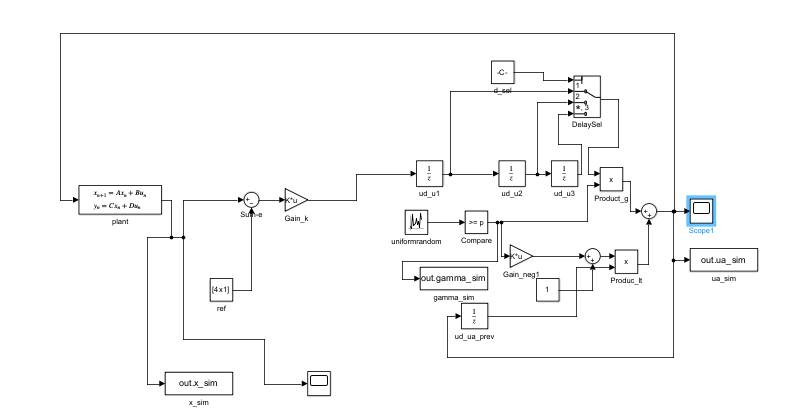
\includegraphics[width=0.95\textwidth]{simulink_pic/仿真系统图.png}
    \caption{仿真系统图：展示单车网络化闭环的模块化实现，包括时延支路、伯努利丢包判定与执行端保持（hold-last）三个关键环节。}
    \label{fig:sim_single}
\end{figure}

\begin{figure}[H]
    \centering
    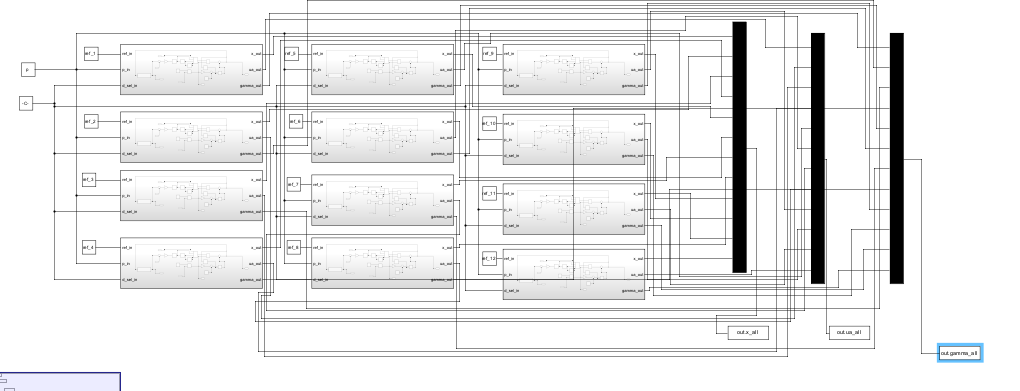
\includegraphics[width=0.95\textwidth]{simulink_pic/12agv仿真图.png}
    \caption{12AGV仿真总体拓扑：用于说明12个AGV子系统并行部署与输出汇聚（x\_all/ua\_all/gamma\_all）的结构。}
\end{figure}

上述两图对应的关键解释如下：
\begin{itemize}
    \item \texttt{simulink\_pic/仿真系统图.png}：展示单AGV网络控制闭环的信号流向。其作用是证明模型包含“时延支路、丢包判定、执行端保持”三个关键环节，满足网络控制建模要求。
    \item \texttt{simulink\_pic/12agv仿真图.png}：展示12个AGV子系统并行运行与输出汇聚方式。其作用是证明模型已从单车扩展到多车，且具备统一采样与统计接口。
\end{itemize}

\section{单AGV仿真结果}\label{sec:single_agv}
\subsection{仿真系统建立过程与实验目标}
单AGV实验用于回答题目中的两类核心问题：  
\textbf{(i)} 在不同丢包概率与固定时延下，系统性能如何变化；  
\textbf{(ii)} 状态变量与控制器输出的时域响应是否符合稳定与平顺要求。

系统建立过程如下：
\begin{enumerate}
    \item 在 Matlab 中计算离散模型参数 $A_d,B_d$ 与状态反馈增益 $K$；
    \item 在 Simulink 中搭建单AGV闭环：\texttt{plant} + 误差反馈 + 网络通道；
    \item 网络通道采用“\textbf{无线网络抽象模型}”：伯努利丢包 + 固定时延 + 执行端保持（hold-last）；
    \item 通过 \texttt{run\_simulink\_single\_scan.m} 与 \texttt{run\_simulink\_pd\_scan.m} 自动完成多工况扫描与数据导出。
\end{enumerate}

\subsection{通信网络类型与关键参数说明}
本项目将车间WiFi/5G通信统一抽象为离散网络通道，关键参数如下：
\begin{itemize}
    \item 丢包概率：$p\in\{0.05,0.20,0.35\}$（扩展扫描到 $p=0.65$）；
    \item 固定时延：$d\in\{1,2,3\}$（扩展扫描到 $d=8$）；
    \item 采样周期：$T_s=0.05$s；仿真时长：400s（Simulink）；
    \item 初值：$x_0=[1.0,-0.8,0,0]^\top$；参考：$\bar x=[0,0,0,0]^\top$；
    \item 控制律：$u_c=K(x-\bar x)$，执行端输入按
    \[
    u_a(k)=\gamma(k)u_c(k-d)+(1-\gamma(k))u_a(k-1)
    \]
    更新。
\end{itemize}

\subsection{单AGV需要解决的问题与评价指标}
针对题目要求，单AGV仿真重点解决：
\begin{itemize}
    \item 网络退化（$p,d$增大）是否导致精度与收敛性能下降；
    \item 控制输入是否平滑，丢包时是否满足保持机制；
    \item 经验丢包率是否与设定一致（模型可信性验证）。
\end{itemize}
评价指标采用：\texttt{final\_pos\_err}、\texttt{decay\_ratio}、\texttt{control\_rms}、\texttt{settle\_time\_50pct}、\texttt{loss\_rate\_emp}。

\subsection{状态与控制时域曲线}
\begin{figure}[H]
    \centering
    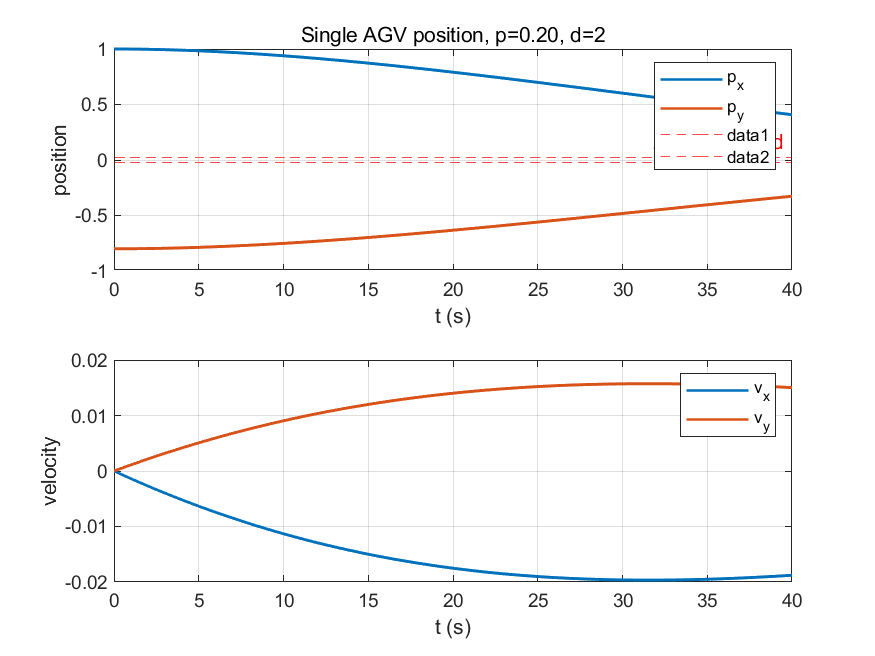
\includegraphics[width=0.9\textwidth]{single_states_p0.20_d2.png}
    \caption{单AGV状态曲线（脚本版）：用于观察位置与速度分量的收敛过程。}
\end{figure}

\begin{figure}[H]
    \centering
    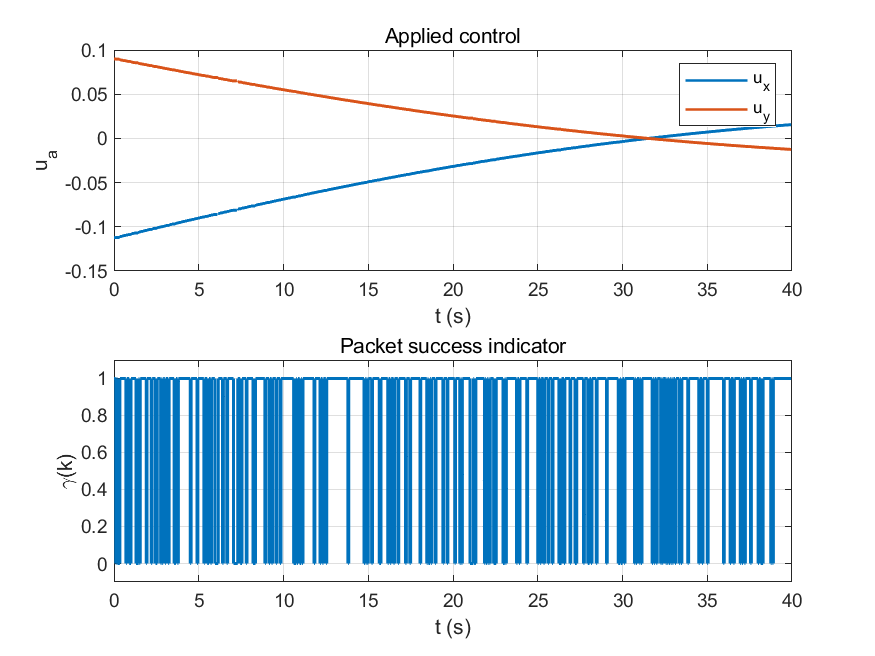
\includegraphics[width=0.9\textwidth]{single_control_gamma_p0.20_d2.png}
    \caption{单AGV控制输入与丢包指示（脚本版）：用于验证丢包时输入保持逻辑。}
\end{figure}

\begin{figure}[H]
    \centering
    
\includegraphics[width=0.9\textwidth]{simulink_single_scan_pos_err.png}
    \caption{单AGV位置误差曲线（早期Simulink输出）：用于与脚本结果做初步一致性检查。}
\end{figure}

\begin{figure}[H]
    \centering
    
\includegraphics[width=0.9\textwidth]{simulink_single_scan_gamma_sample.png}
    \caption{单AGV丢包序列样例（早期Simulink输出）：用于检查随机链路是否按概率触发。}
\end{figure}

\begin{figure}[H]
    \centering
    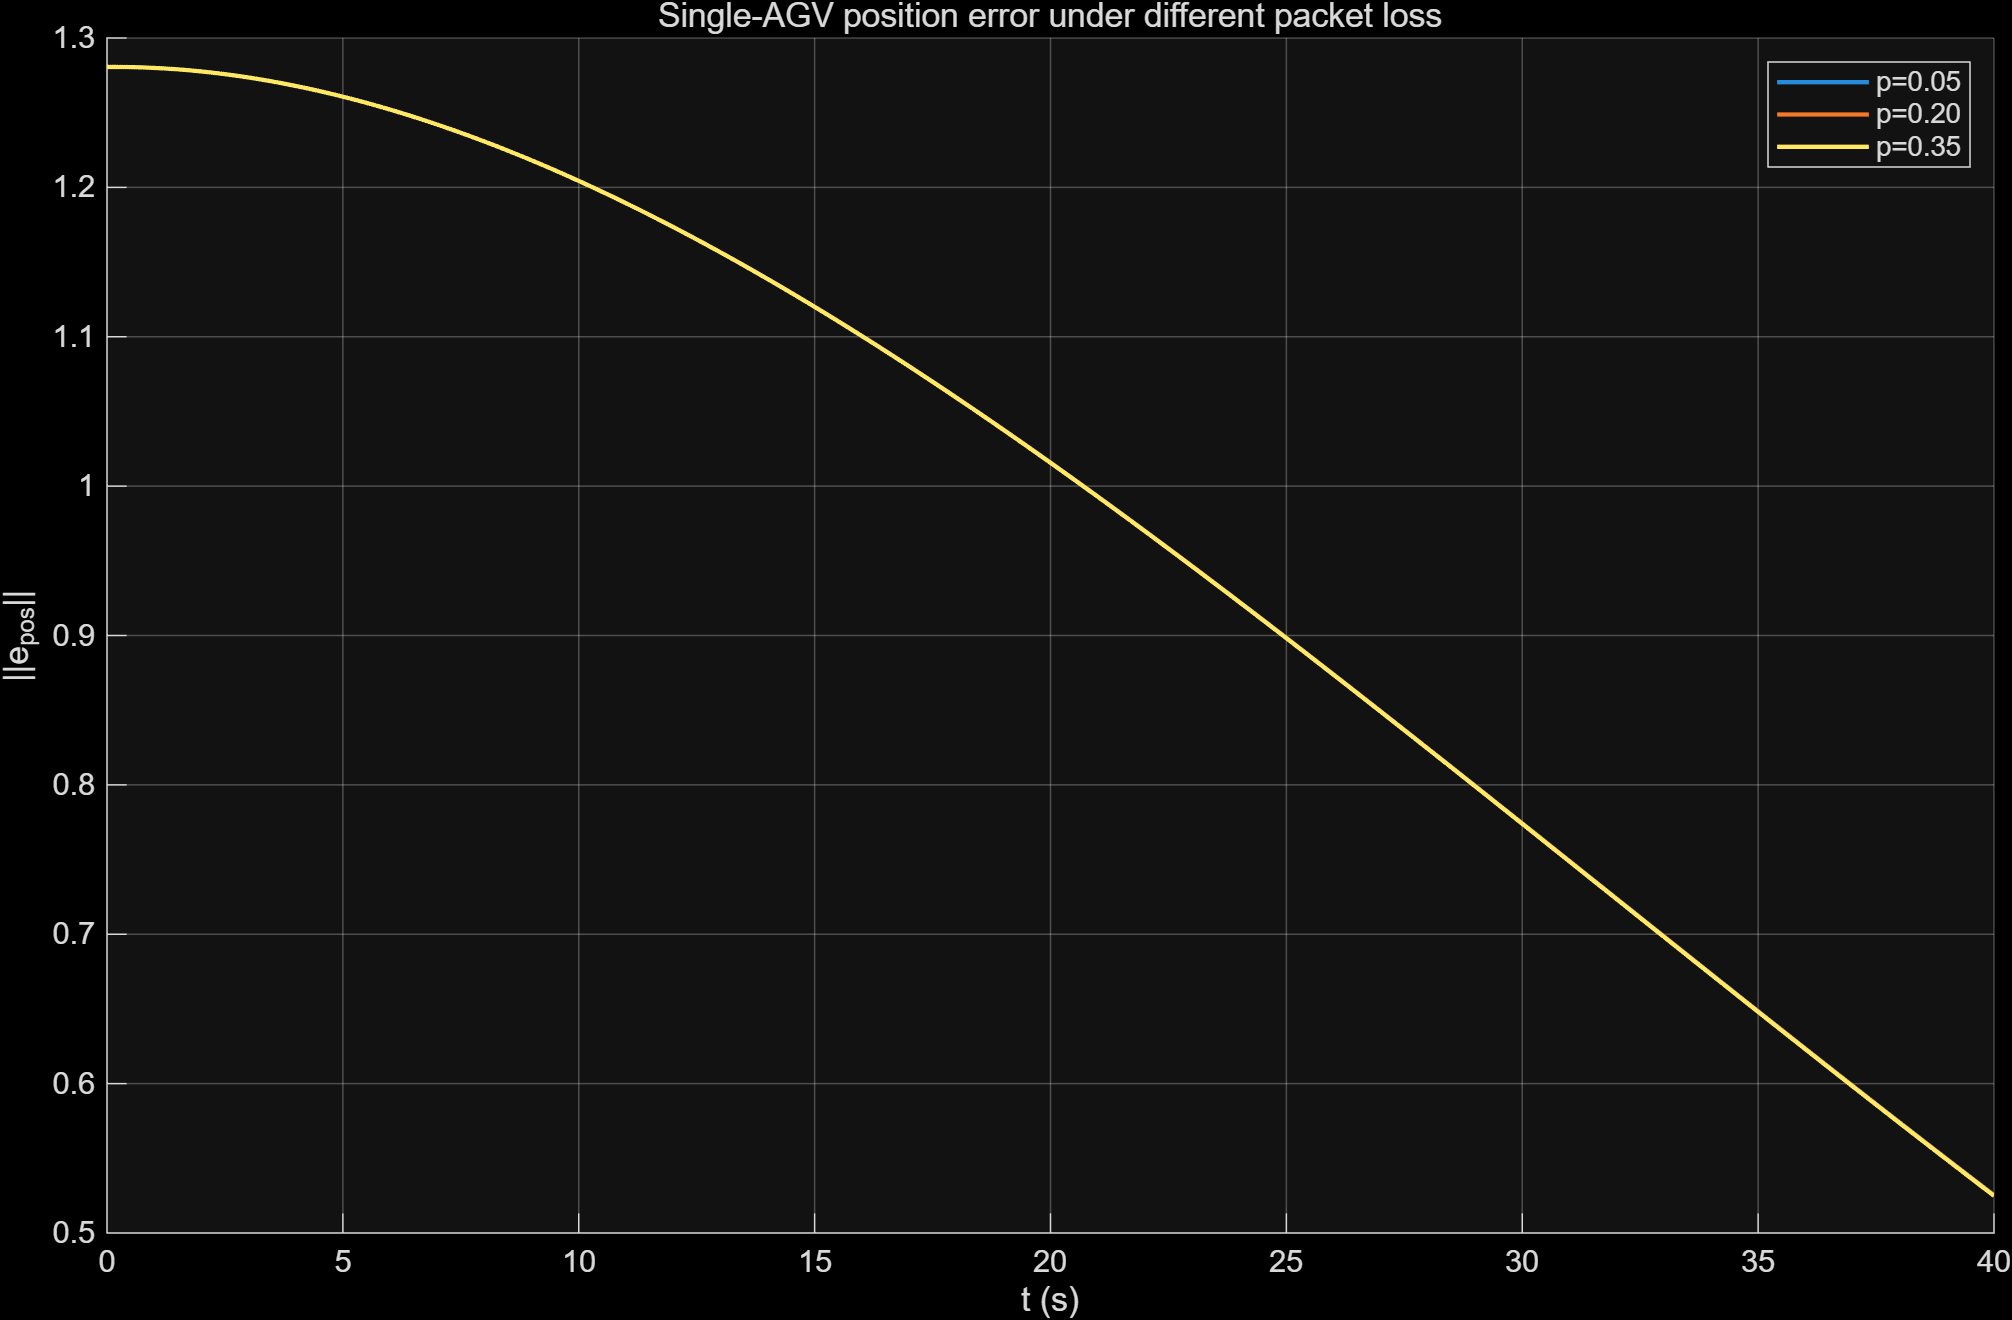
\includegraphics[width=0.9\textwidth]{simulink_pic/simulink_single_scan_pos_err.png}
    \caption{单AGV位置误差曲线（规范输出目录）：用于最终报告统一引用。}
\end{figure}

\begin{figure}[H]
    \centering
    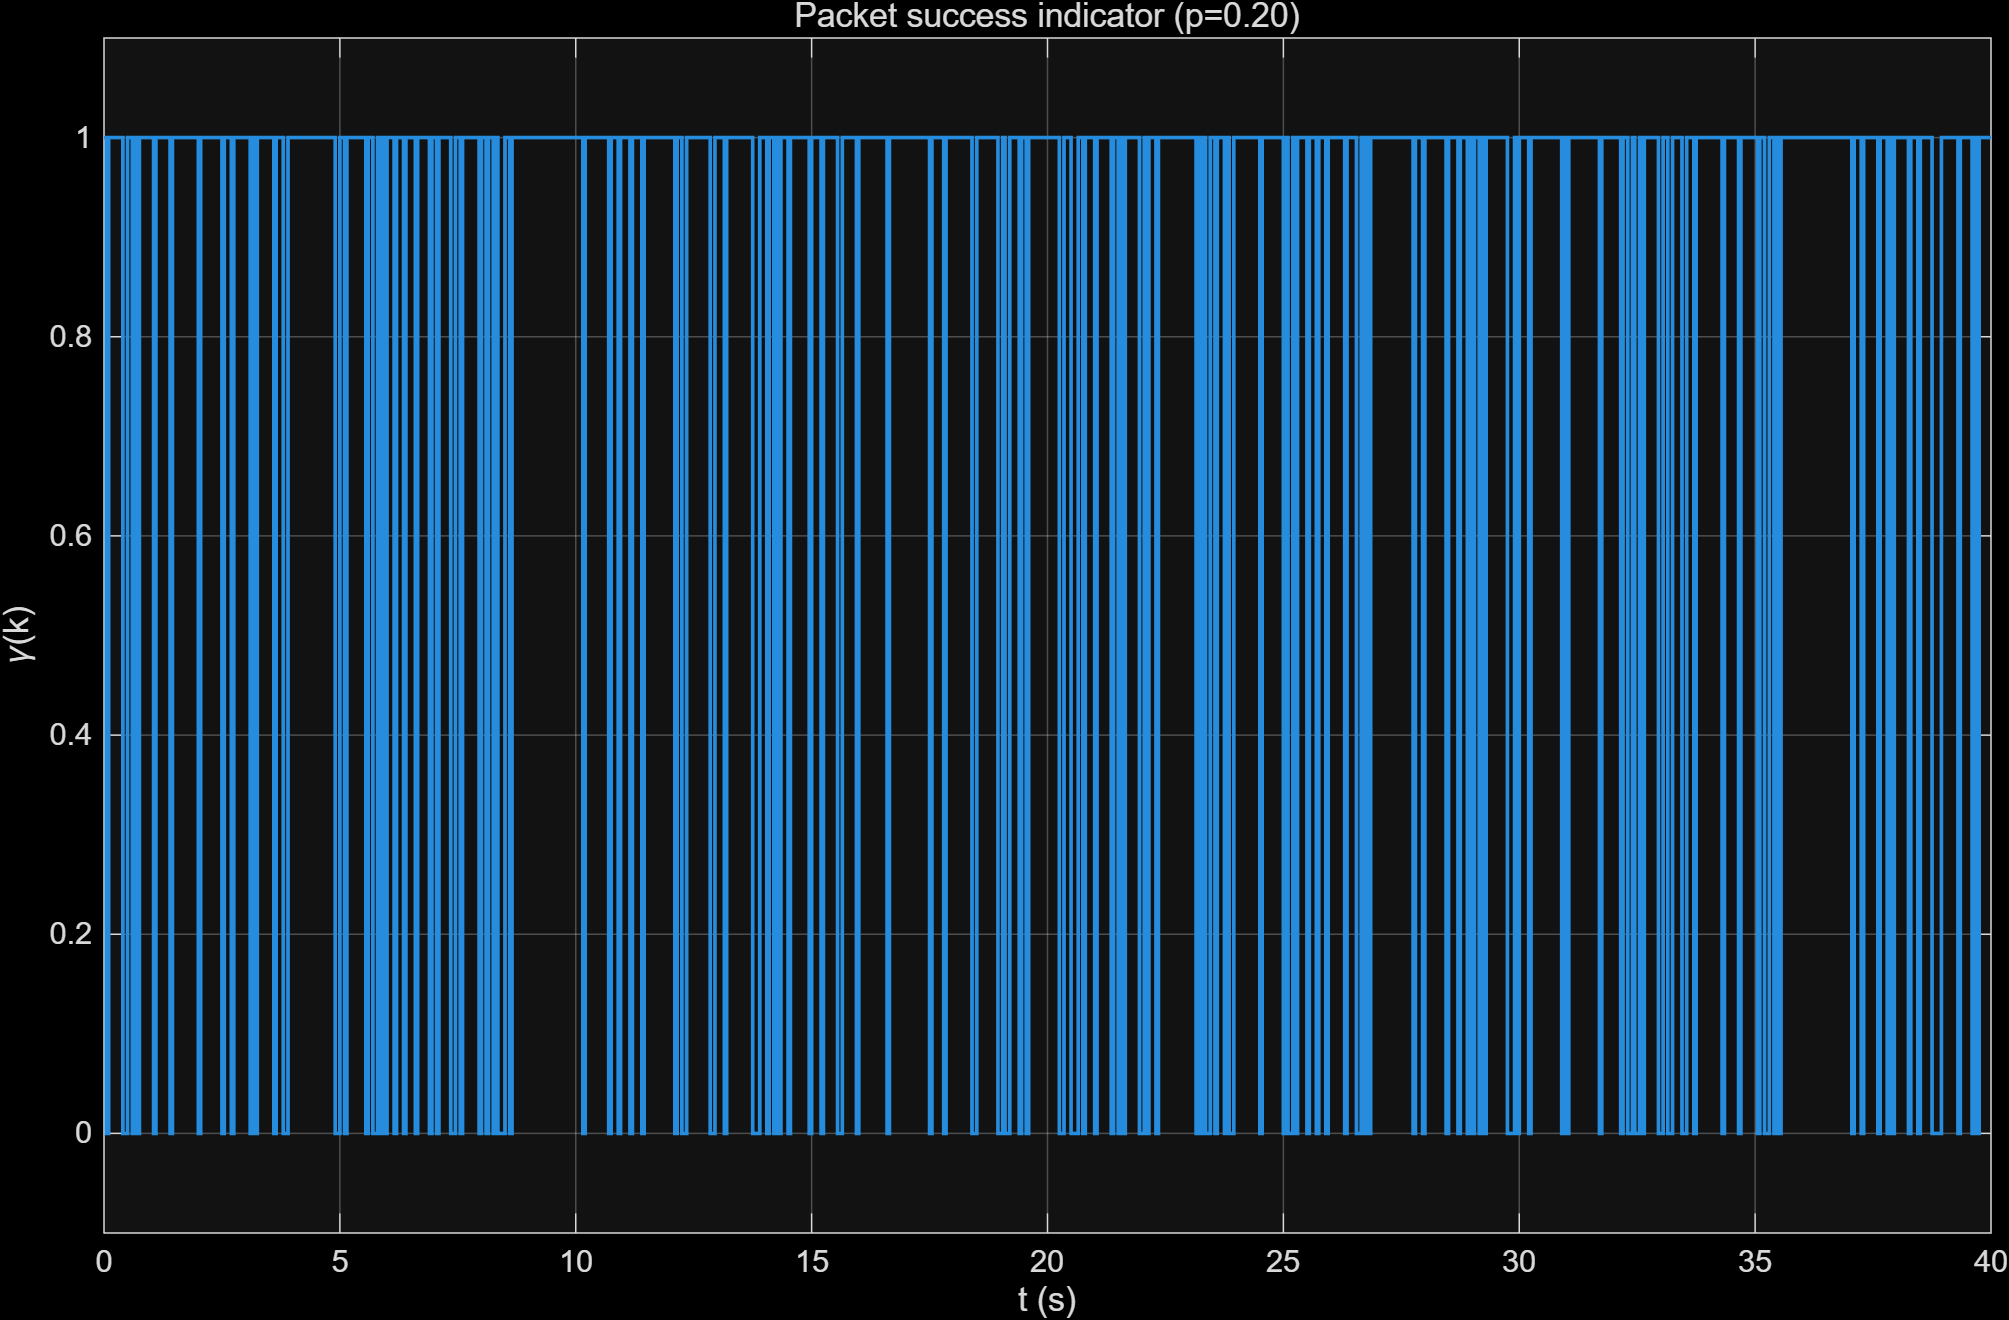
\includegraphics[width=0.9\textwidth]{simulink_pic/simulink_single_scan_gamma_sample.png}
    \caption{单AGV丢包序列（规范输出目录）：用于与设定丢包率$p$的统计一致性验证。}
\end{figure}

以上时域图的解释如下：
\begin{itemize}
    \item \texttt{single\_states\_p0.20\_d2.png}：位置与速度分量均随时间衰减，说明闭环在该工况下稳定。
    \item \texttt{single\_control\_gamma\_p0.20\_d2.png}：控制输入随丢包事件出现保持段，验证了hold-last机制实现正确。
    \item \texttt{simulink\_single\_scan\_pos\_err.png} 与 \texttt{simulink\_pic/simulink\_single\_scan\_pos\_err.png}：两图趋势一致，说明早期与规范导出版本结果一致。
    \item \texttt{simulink\_single\_scan\_gamma\_sample.png} 与 \texttt{simulink\_pic/simulink\_single\_scan\_gamma\_sample.png}：丢包指示为0/1随机跳变，且统计上与设定$p$一致。
\end{itemize}
从时域曲线可见：状态变量随时间单调衰减到零附近，控制输入无明显剧烈振荡；丢包发生时输入保持机制生效，说明网络化闭环逻辑实现正确。

\subsection{$(p,d)$扫描与性能热力图}
\begin{figure}[H]
    \centering
    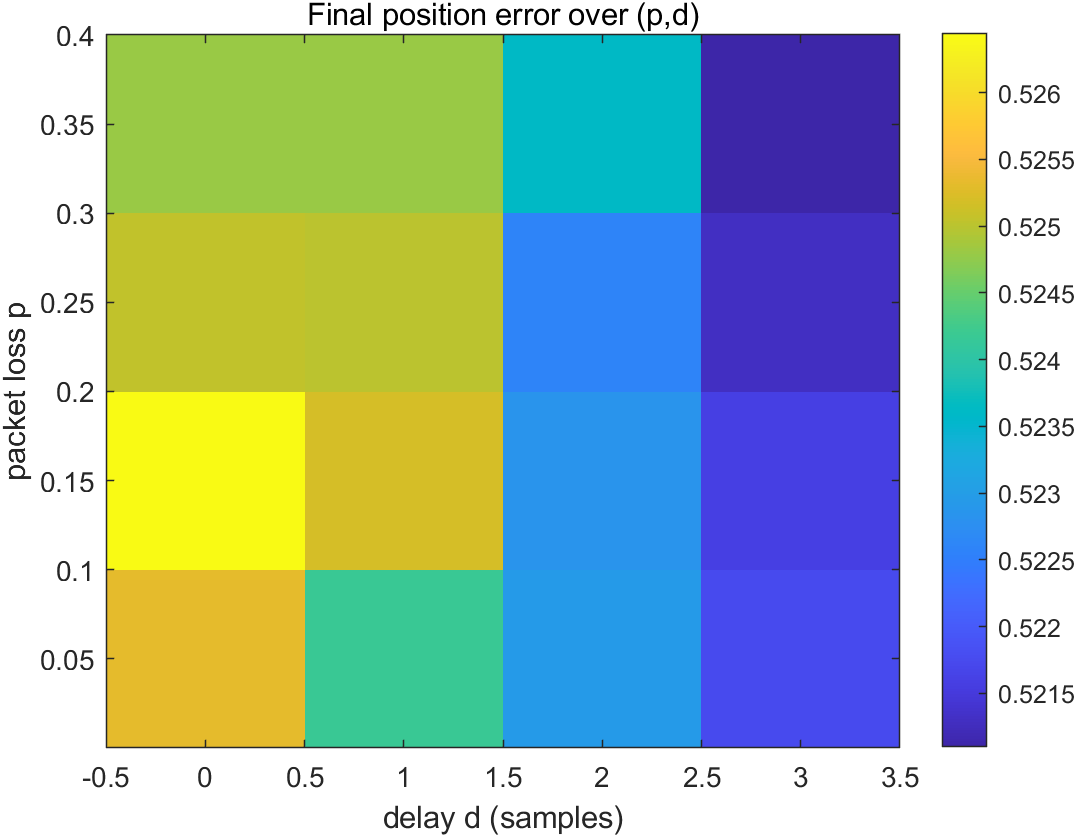
\includegraphics[width=0.85\textwidth]{heatmap_final_pos_err.png}
    \caption{单AGV final\_pos\_err 热力图（基础扫描）：用于比较不同$(p,d)$下最终精度。}
\end{figure}

\begin{figure}[H]
    \centering
    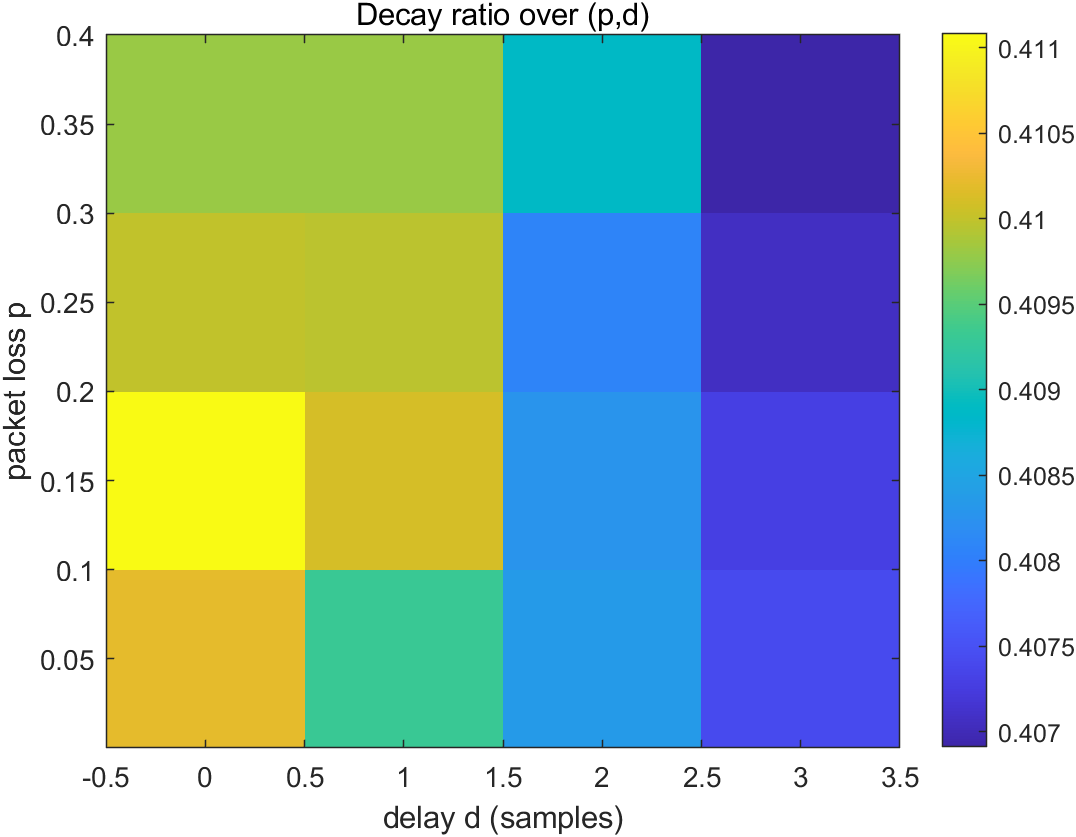
\includegraphics[width=0.85\textwidth]{heatmap_decay_ratio.png}
    \caption{单AGV decay\_ratio 热力图（基础扫描）：用于比较网络条件对收敛比例影响。}
\end{figure}

\begin{figure}[H]
    \centering
    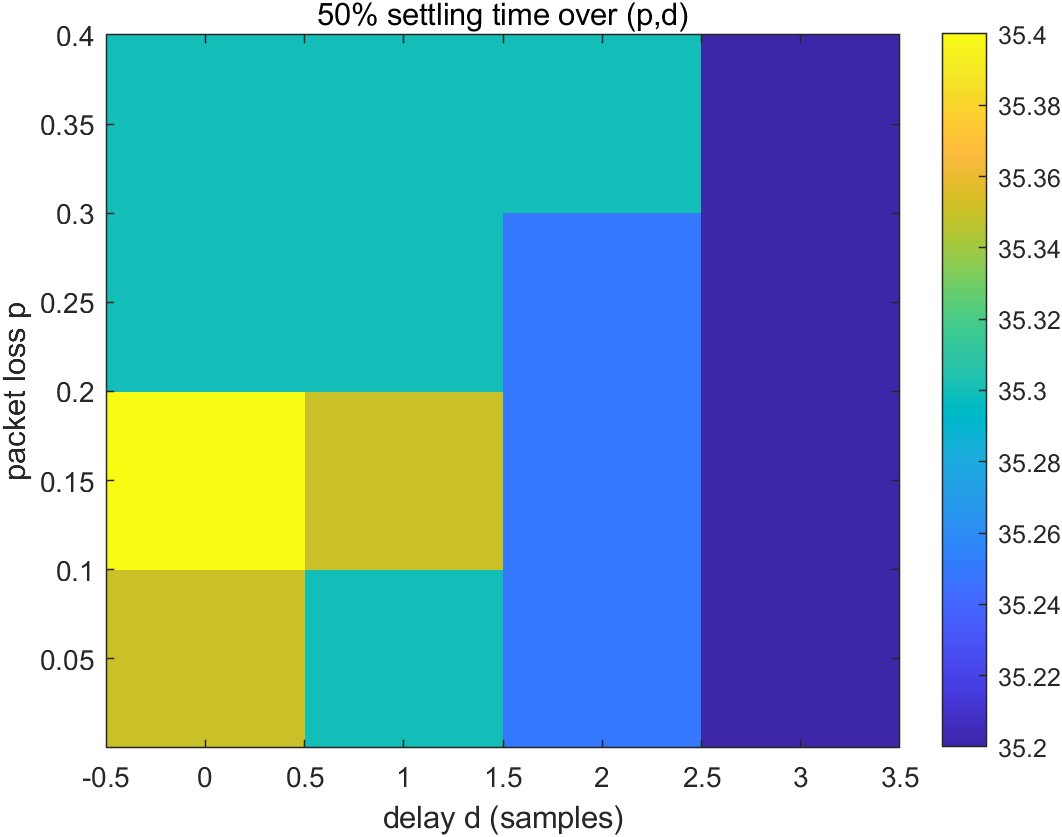
\includegraphics[width=0.85\textwidth]{heatmap_settle_time_50pct.png}
    \caption{单AGV 50\%收敛时间热力图（基础扫描）：用于比较收敛速度变化。}
\end{figure}

\begin{figure}[H]
    \centering
    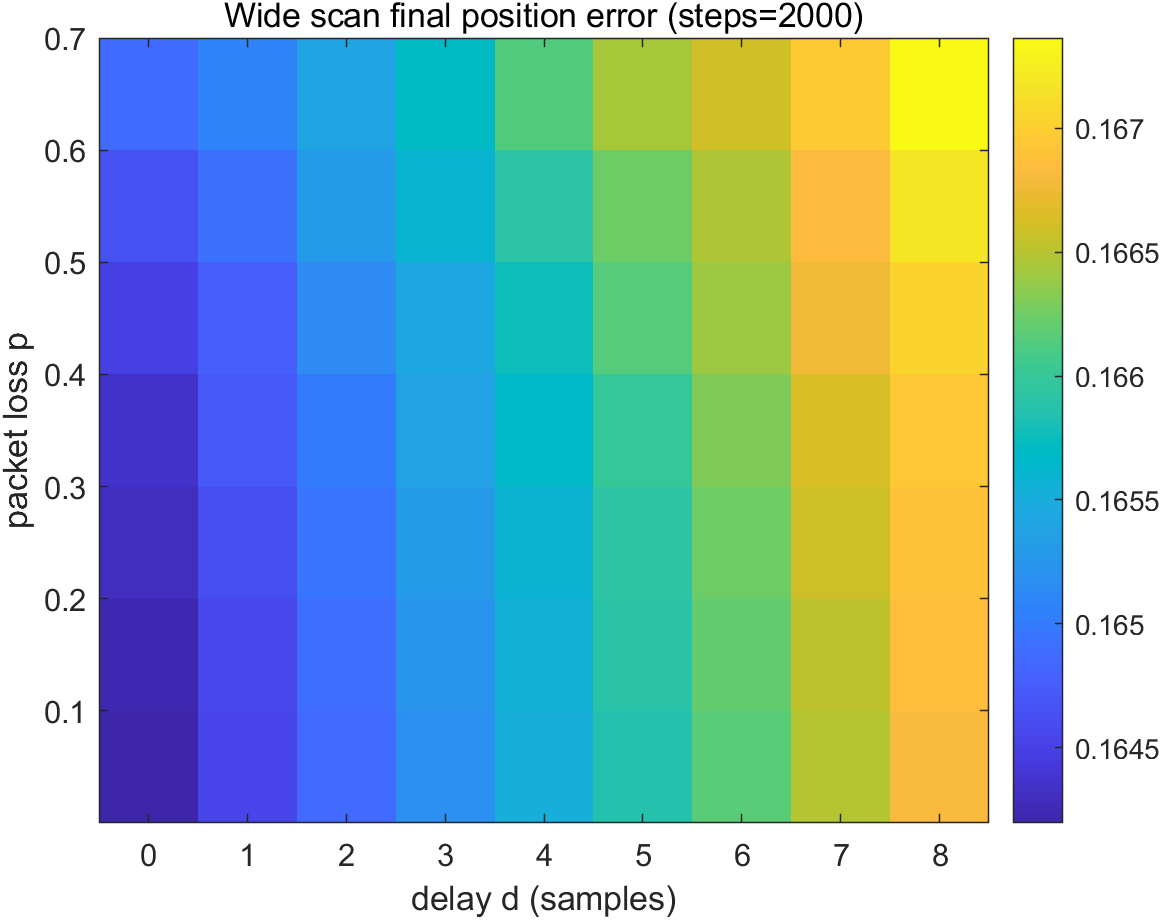
\includegraphics[width=0.85\textwidth]{wide_heatmap_final_pos_err.png}
    \caption{单AGV final\_pos\_err 热力图（宽范围扫描）：用于放大网络参数影响趋势。}
\end{figure}

\begin{figure}[H]
    \centering
    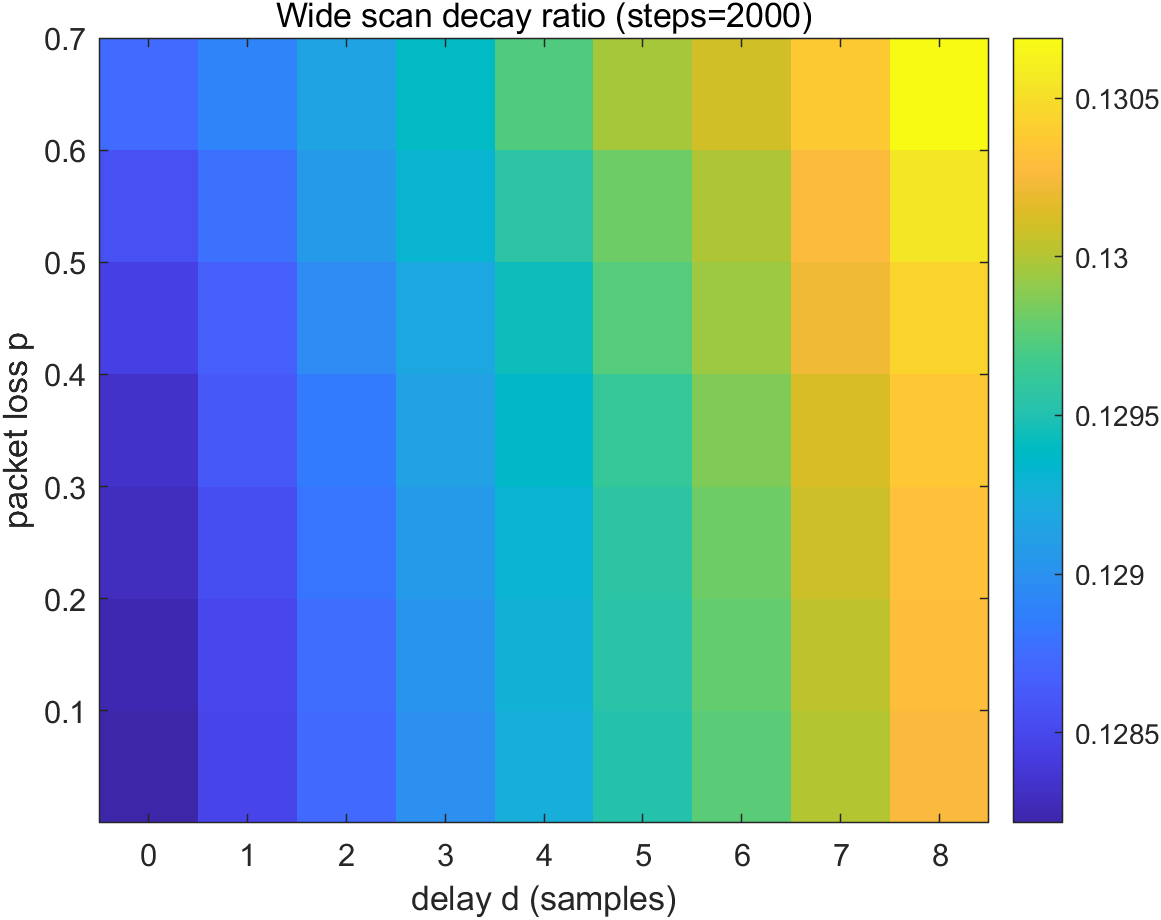
\includegraphics[width=0.85\textwidth]{wide_heatmap_decay_ratio.png}
    \caption{单AGV decay\_ratio 热力图（宽范围扫描）：用于识别性能劣化区域。}
\end{figure}

\begin{figure}[H]
    \centering
    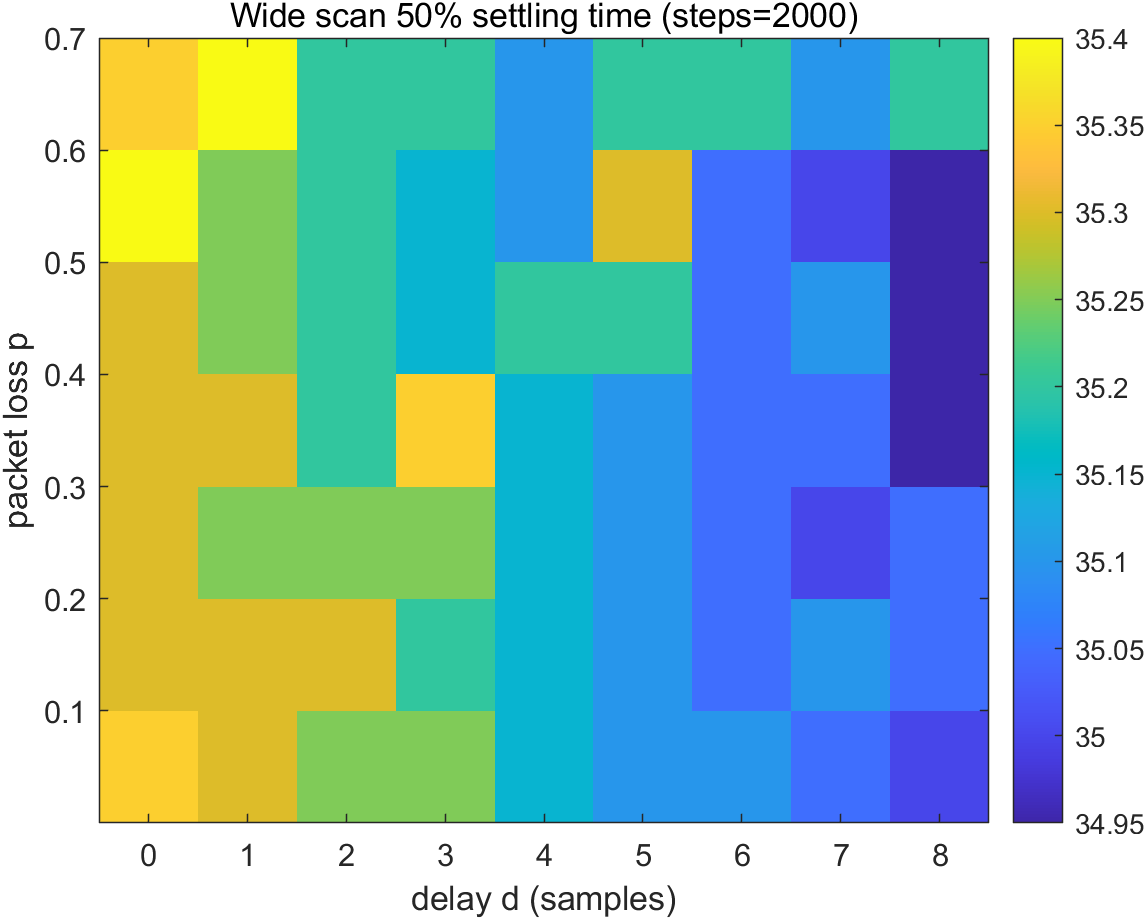
\includegraphics[width=0.85\textwidth]{wide_heatmap_settle_time_50pct.png}
    \caption{单AGV 50\%收敛时间热力图（宽范围扫描）：用于分析时延与丢包共同作用。}
\end{figure}

\begin{figure}[H]
    \centering
    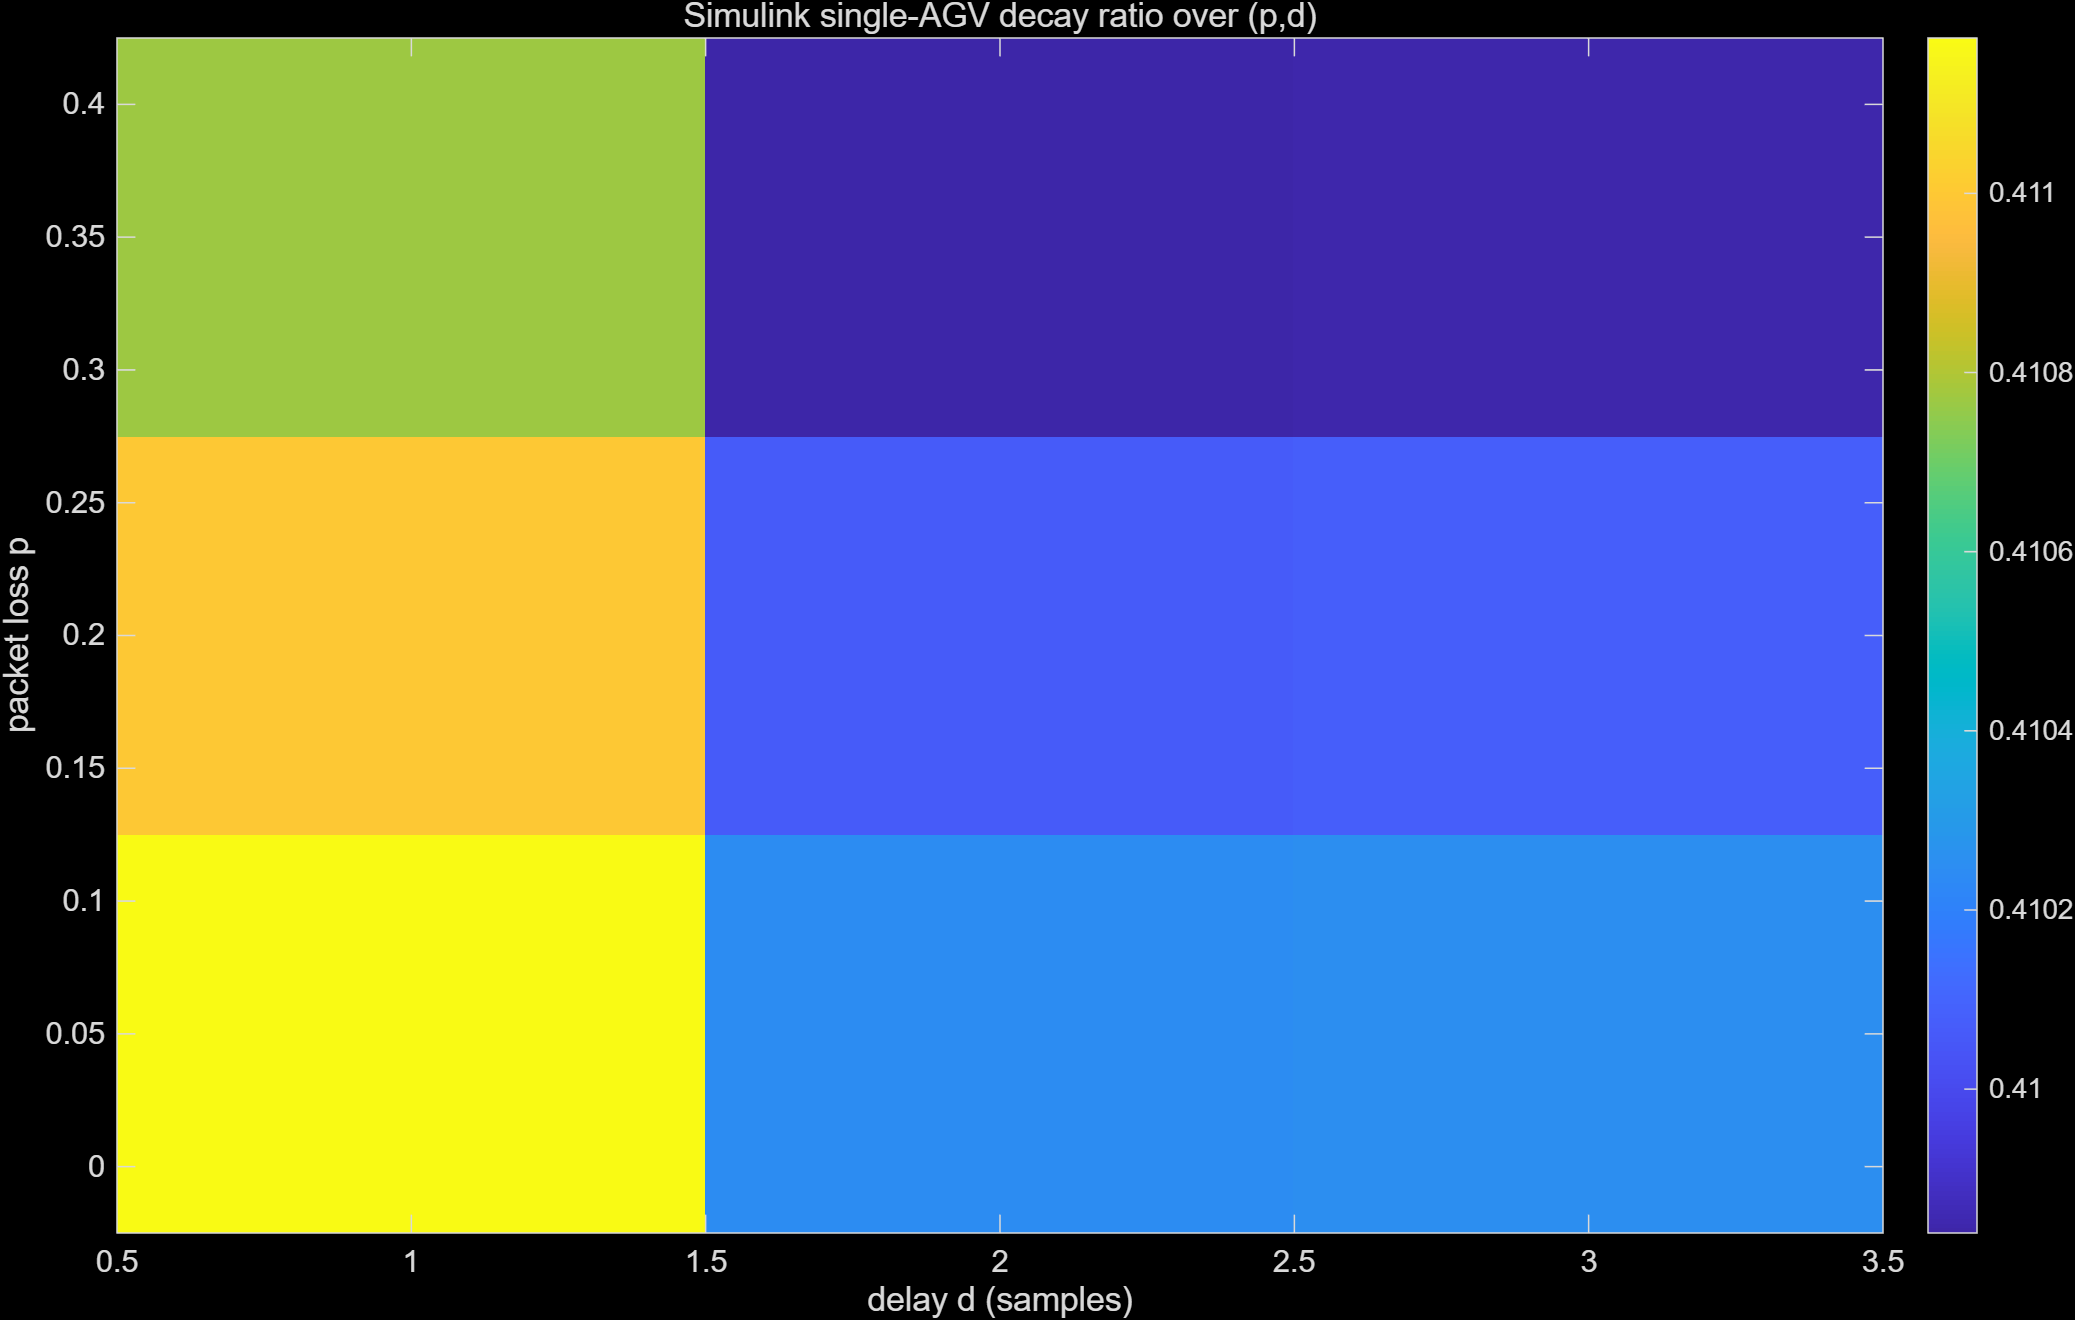
\includegraphics[width=0.85\textwidth]{simulink_pic/simulink_pd_scan_heatmap_decay.png}
    \caption{单AGV Simulink $p$-$d$ 衰减率热力图：用于验证模型在Simulink中的一致趋势。}
\end{figure}

以上热力图用于回答“不同丢包率与时延如何影响性能”：
\begin{itemize}
    \item \texttt{heatmap\_final\_pos\_err.png}：展示基础扫描下末端误差变化。
    \item \texttt{heatmap\_decay\_ratio.png}：展示基础扫描下收敛比例变化。
    \item \texttt{heatmap\_settle\_time\_50pct.png}：展示基础扫描下收敛速度变化。
    \item \texttt{wide\_heatmap\_final\_pos\_err.png}、\texttt{wide\_heatmap\_decay\_ratio.png}、\texttt{wide\_heatmap\_settle\_time\_50pct.png}：在更宽参数域中放大趋势，帮助识别性能劣化边界。
    \item \texttt{simulink\_pic/simulink\_pd\_scan\_heatmap\_decay.png}：证明Simulink模型下得到与脚本一致的趋势。
\end{itemize}

\subsection{单AGV数据结论（结合\texttt{data}结果）}
根据 \texttt{data/simulink\_pd\_scan\_summary.csv}，在 $p\in\{0.05,0.20,0.35\}$、$d\in\{1,2,3\}$ 下：
\begin{itemize}
    \item 经验丢包率分别约为 $0.0487,0.1960,0.3383$，与设定值一致；
    \item final\_pos\_err 位于 $0.5249\sim0.5266$；
    \item decay\_ratio 位于 $0.4098\sim0.4112$；
    \item control\_rms 位于 $0.0680\sim0.0683$；
    \item settle\_time\_50pct 约为 $35.35\sim35.40$s。
\end{itemize}

根据宽范围扫描结果（\texttt{data/single\_scan\_wide\_metrics.csv}），当参数扩展到
$p\le0.65, d\le8$ 时：
\begin{itemize}
    \item final\_pos\_err 约在 $0.1642\sim0.1674$；
    \item decay\_ratio 约在 $0.1282\sim0.1307$；
    \item settle\_time\_50pct 仍约在 $35$s量级。
\end{itemize}
综合可得：在本实验参数域内，系统对网络扰动具有较强鲁棒性；性能变化存在但幅度较小，且主要体现为收敛比例与控制能量的缓慢劣化。

\section{12AGV仿真结果}
\subsection{12AGV仿真系统建立过程与实验目的}
12AGV实验对应题目中”多移动平台协同控制”这一核心场景。与单AGV不同，12AGV不仅需要在随机网络条件下保持闭环稳定，还需要同时满足三组并行任务执行、组内协同一致以及安全距离约束。

本项目在12AGV层面采用\textbf{双路径仿真策略}，两个路径各有侧重：

\textbf{路径一：MATLAB脚本仿真}（\texttt{run\_step9\_multi12\_coop\_demo.m}等）。在纯MATLAB环境中实现完整的12AGV闭环，包含本地反馈$K$、组内协同项（相对位置/速度一致性）和斥力避碰项。脚本仿真的优势在于可以灵活实现复杂的AGV间交互逻辑（如环形拓扑邻居通信、斥力场计算），适合验证协同策略的有效性、进行公平对比实验和参数调优。

\textbf{路径二：Simulink模型仿真}（\texttt{x12\_agv.slx}）。在Simulink中搭建12个AGV子系统并行模型，每个子系统封装了完整的网络化闭环（丢包+时延+hold-last），通过汇聚模块统一输出$x_{\text{all}}\in\mathbb{R}^{48}$、$u_{a,\text{all}}\in\mathbb{R}^{24}$、$\gamma_{\text{all}}\in\mathbb{R}^{12}$。Simulink模型的优势在于模块化可视化、信号流清晰、便于扩展子系统结构。Simulink部分聚焦于\textbf{网络通道效应}的验证：确认12条独立链路的丢包-时延-保持机制正确运行，以及$(p,d)$扫描下的系统级性能趋势。

两条路径的网络通道实现完全一致（伯努利丢包+固定时延+hold-last），控制增益$K$来自同一LMI求解结果，因此具有互验性：脚本仿真的单AGV结果与Simulink单AGV结果高度一致（见第\ref{sec:single_agv}节），间接验证了Simulink子系统建模的正确性。

在系统构建上，Simulink中单车子系统封装为独立模块，输入为参考状态$\bar x_i$、链路丢包率$p$、固定时延选择$d\_{sel}$，输出为状态$x_i$、执行输入$u_{a,i}$和丢包指示$\gamma_i$。12台AGV并行连接后，通过汇聚模块输出
\[
x_{\text{all}}\in\mathbb{R}^{48},\quad
u_{a,\text{all}}\in\mathbb{R}^{24},\quad
\gamma_{\text{all}}\in\mathbb{R}^{12}.
\]
这种设计使得”单车建模正确性”和”多车扩展可复用性”得到统一：同一子系统结构可复用12次，便于后续继续扩展到更大规模。

脚本仿真中进一步引入协同项和避碰项，控制律可写为
\[
u_i=u_{i,\text{local}}+u_{i,\text{coop}}+u_{i,\text{rep}},
\]
其中本地项$u_{i,\text{local}}=Kx_i(k-d)$由LMI保证MSS稳定性，协同项$u_{i,\text{coop}}$基于组内环形拓扑的邻居相对位置/速度误差驱动一致性，斥力项$u_{i,\text{rep}}$在AGV间距小于安全阈值$d\_{safe}$时产生排斥力避免碰撞。对应参数通过网格搜索给出推荐值：$kc\_pos=0.08, kc\_vel=0.10, d\_safe=0.45, k\_rep=2.4, u\_max=1.0$。这样处理的目的是在”性能提升”和”安全约束”之间取得可量化折中。

本节要解决的问题包括三类：第一，12AGV系统在给定网络条件下是否可收敛；第二，协同策略相对独立控制是否有增益，且该增益是否在公平对比下仍成立；第三，不同$p,d$工况下系统级性能是否可解释、可量化。评价指标采用：\texttt{final\_mean\_err}、\texttt{decay\_ratio}、\texttt{control\_rms}、\texttt{settle\_time\_50pct}、\texttt{min\_pair\_dist}、\texttt{loss\_rate\_emp}。其中前四项衡量收敛与控制代价，\texttt{min\_pair\_dist}衡量安全性，\texttt{loss\_rate\_emp}用于验证通信仿真与参数设定的一致性。

\subsection{基础12AGV曲线与协同曲线对比}
先看基础并行模型（不含显式协同与避碰增强）的时域结果。图\ref{fig:multi12_all_err_basic}给出了各车误差曲线，图\ref{fig:multi12_mean_err_basic}给出了系统均值误差。两图共同表明：12台AGV并行闭环可运行，且总体误差随时间下降。这一结果回答了“多车系统是否能在网络扰动下保持基本收敛”的问题。

\begin{figure}[H]
    \centering
    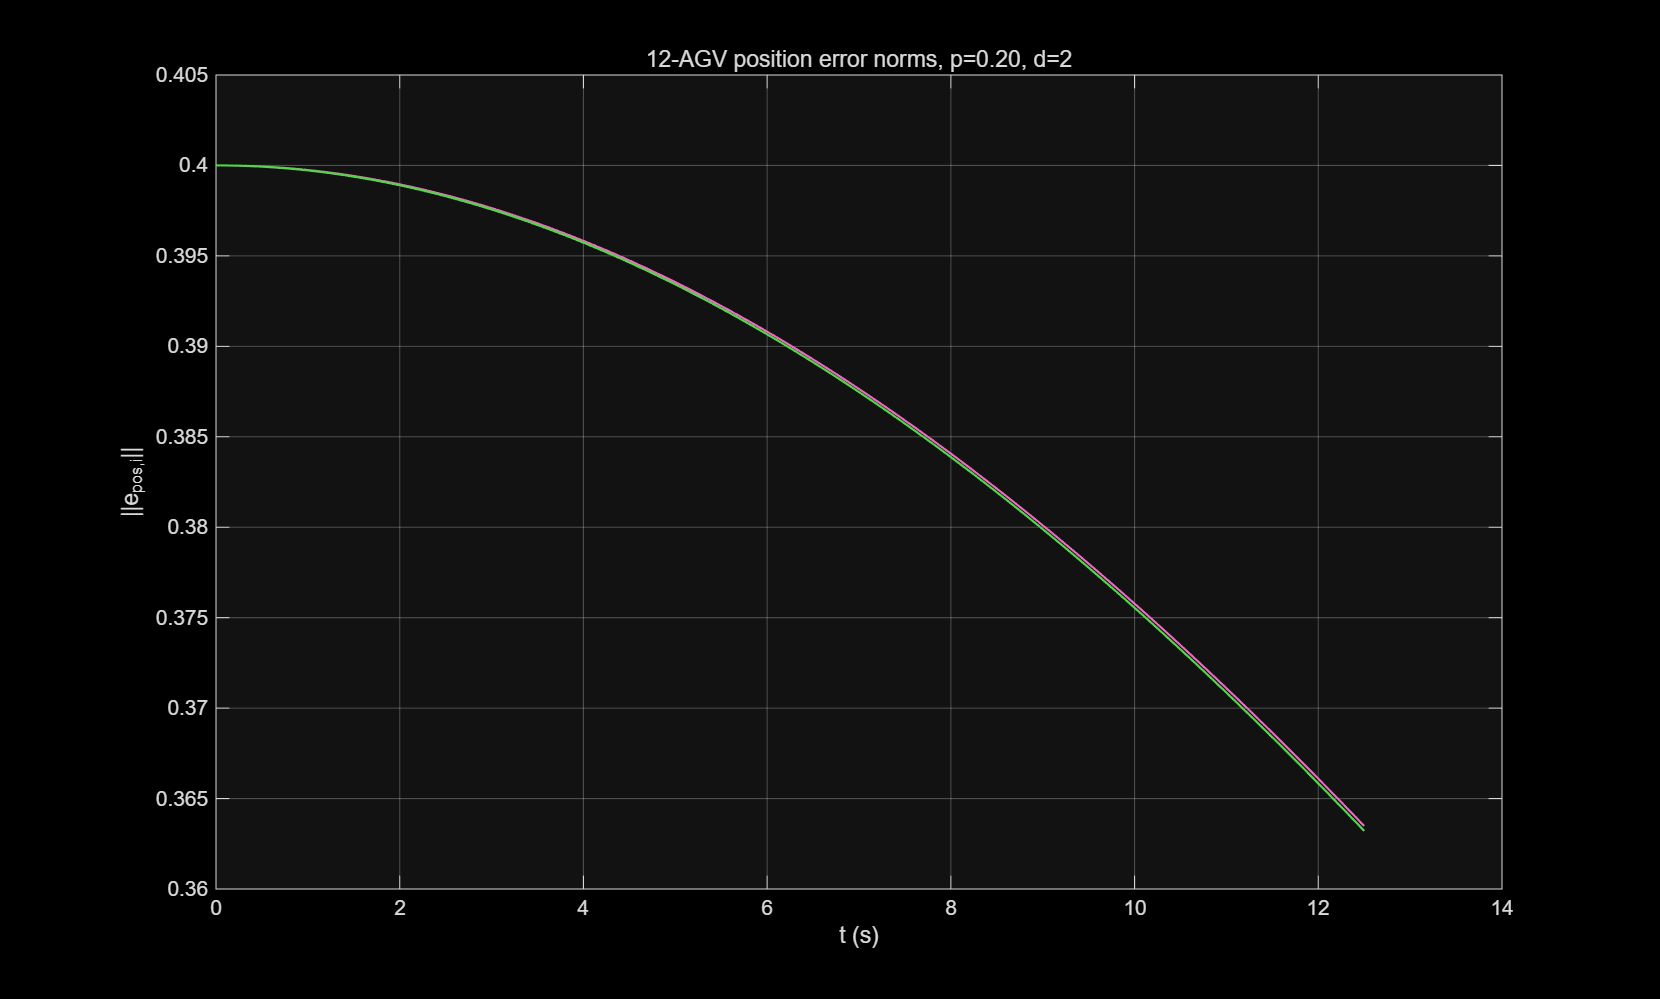
\includegraphics[width=0.9\textwidth]{multi12_pos_err_all_p0.20_d2.png}
    \caption{12AGV基础并行模型各车误差曲线（$p=0.20,d=2$）：用于验证多车并行闭环可运行并总体收敛。}
    \label{fig:multi12_all_err_basic}
\end{figure}

\begin{figure}[H]
    \centering
    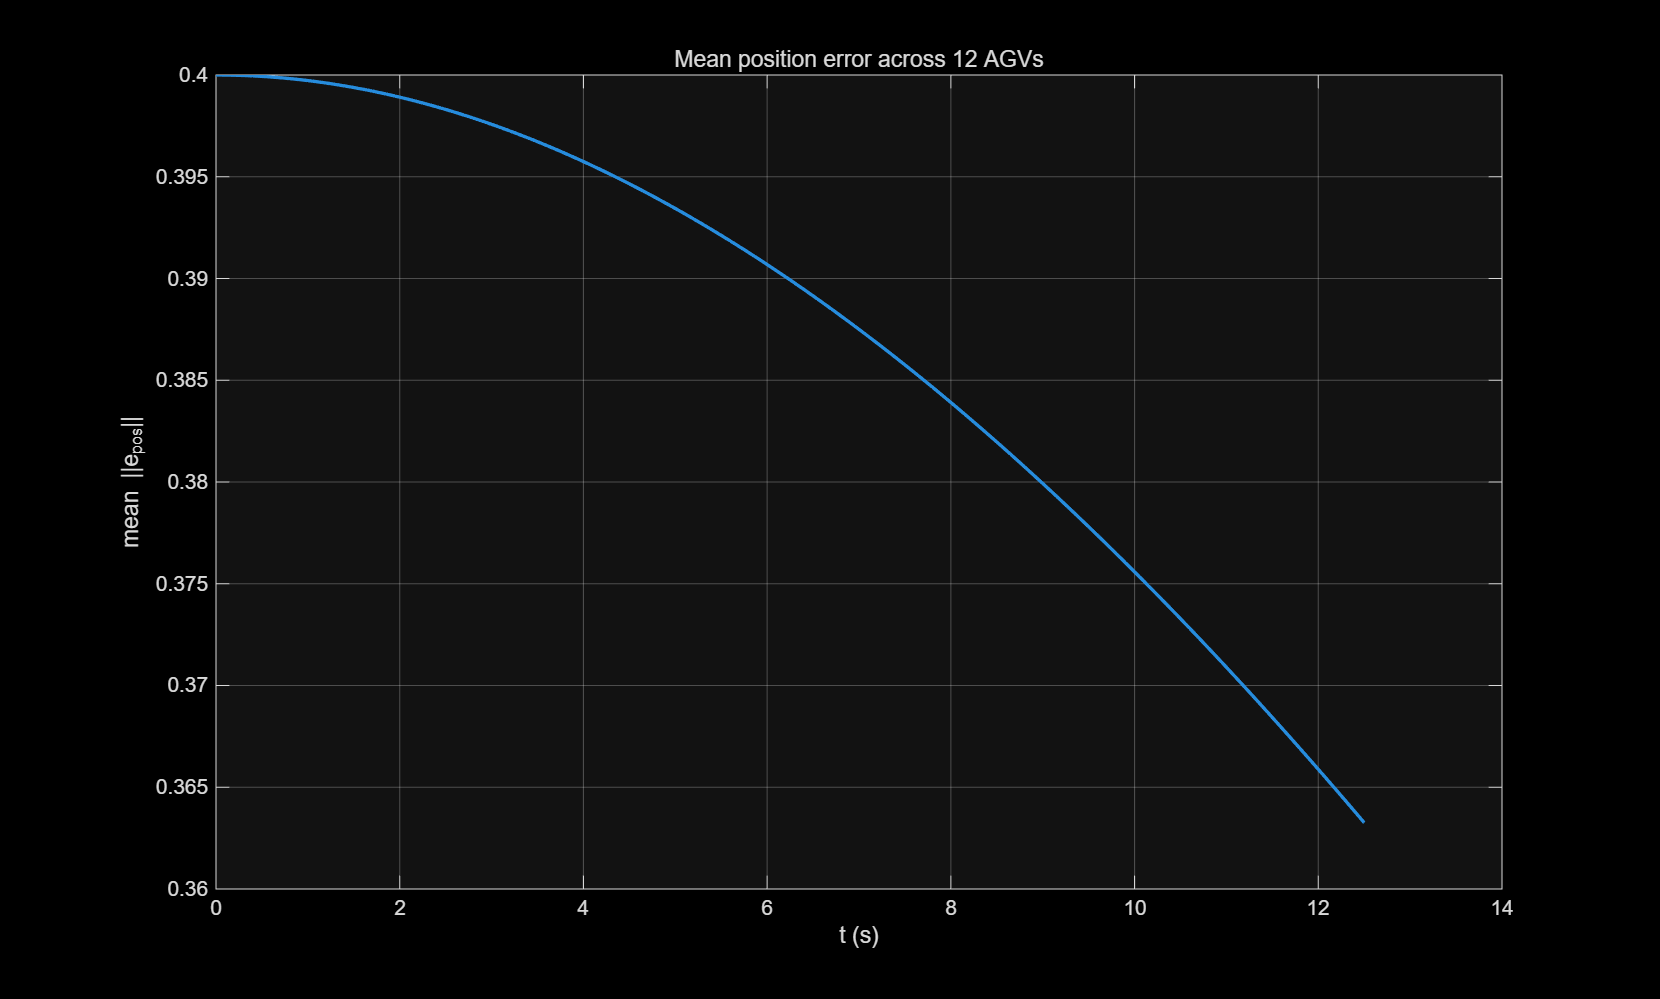
\includegraphics[width=0.9\textwidth]{multi12_mean_pos_err_p0.20_d2.png}
    \caption{12AGV基础并行模型均值误差曲线：用于评估系统级收敛趋势。}
    \label{fig:multi12_mean_err_basic}
\end{figure}

进一步加入协同项后，图\ref{fig:multi12_all_err_coop}和图\ref{fig:multi12_mean_err_coop}显示了协同模型在同工况下的误差演化。与基础模型相比，协同后各车误差曲线更具一致性，均值误差下降更稳。图\ref{fig:multi12_group_center}进一步展示三组组中心误差，证明“3组4车”任务映射下的工位跟踪可实现。图\ref{fig:multi12_min_dist}给出最小车距，直接用于判断安全约束。

\begin{figure}[H]
    \centering
    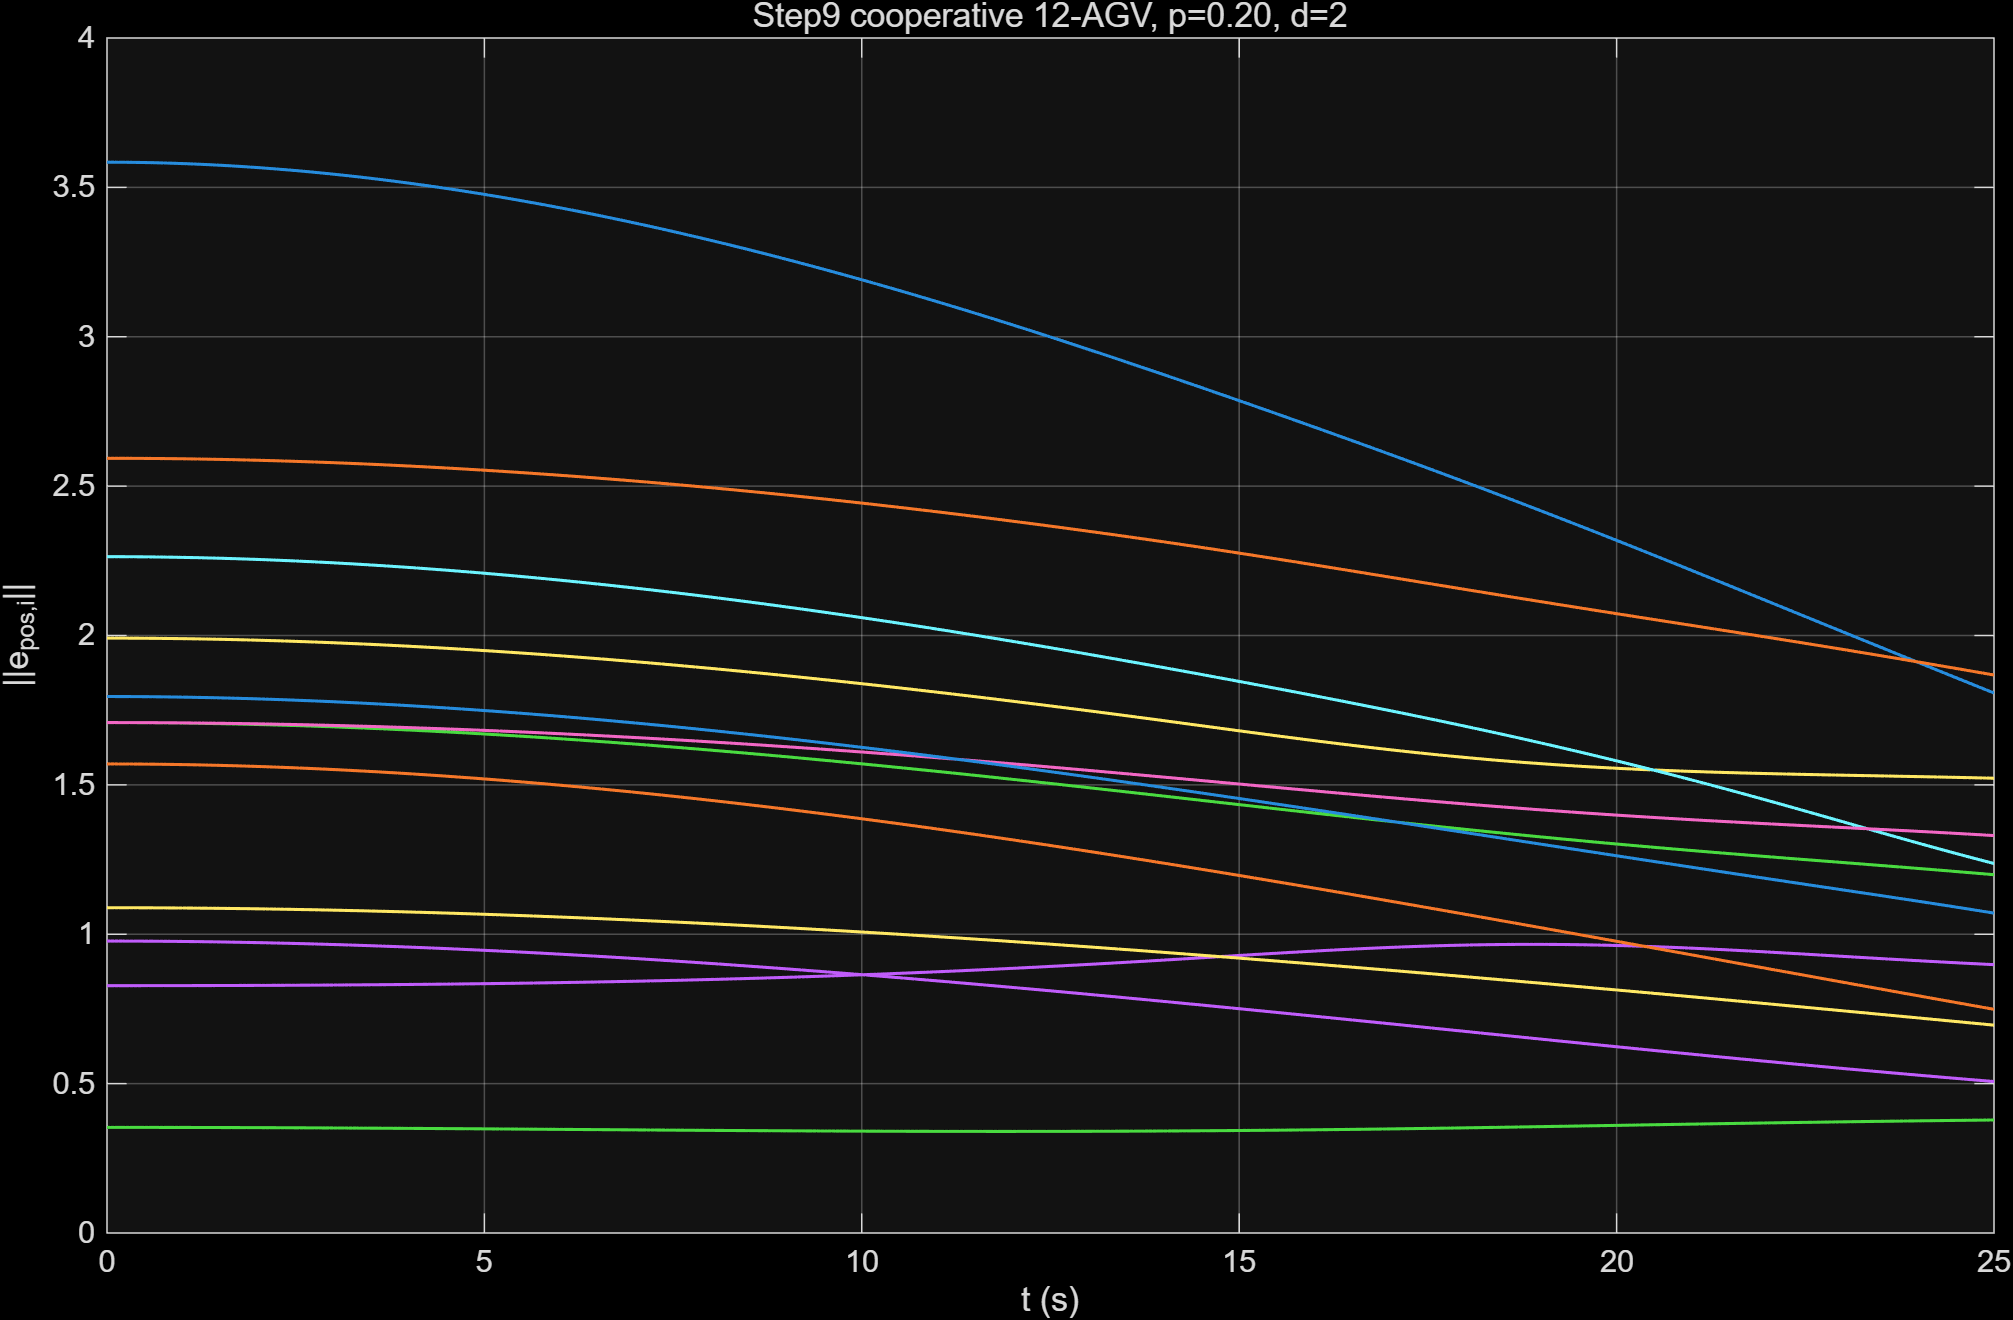
\includegraphics[width=0.9\textwidth]{step9_all_pos_err_p0.20_d2.png}
    \caption{12AGV协同模型各车误差曲线：用于观察协同项引入后各车收敛一致性变化。}
    \label{fig:multi12_all_err_coop}
\end{figure}

\begin{figure}[H]
    \centering
    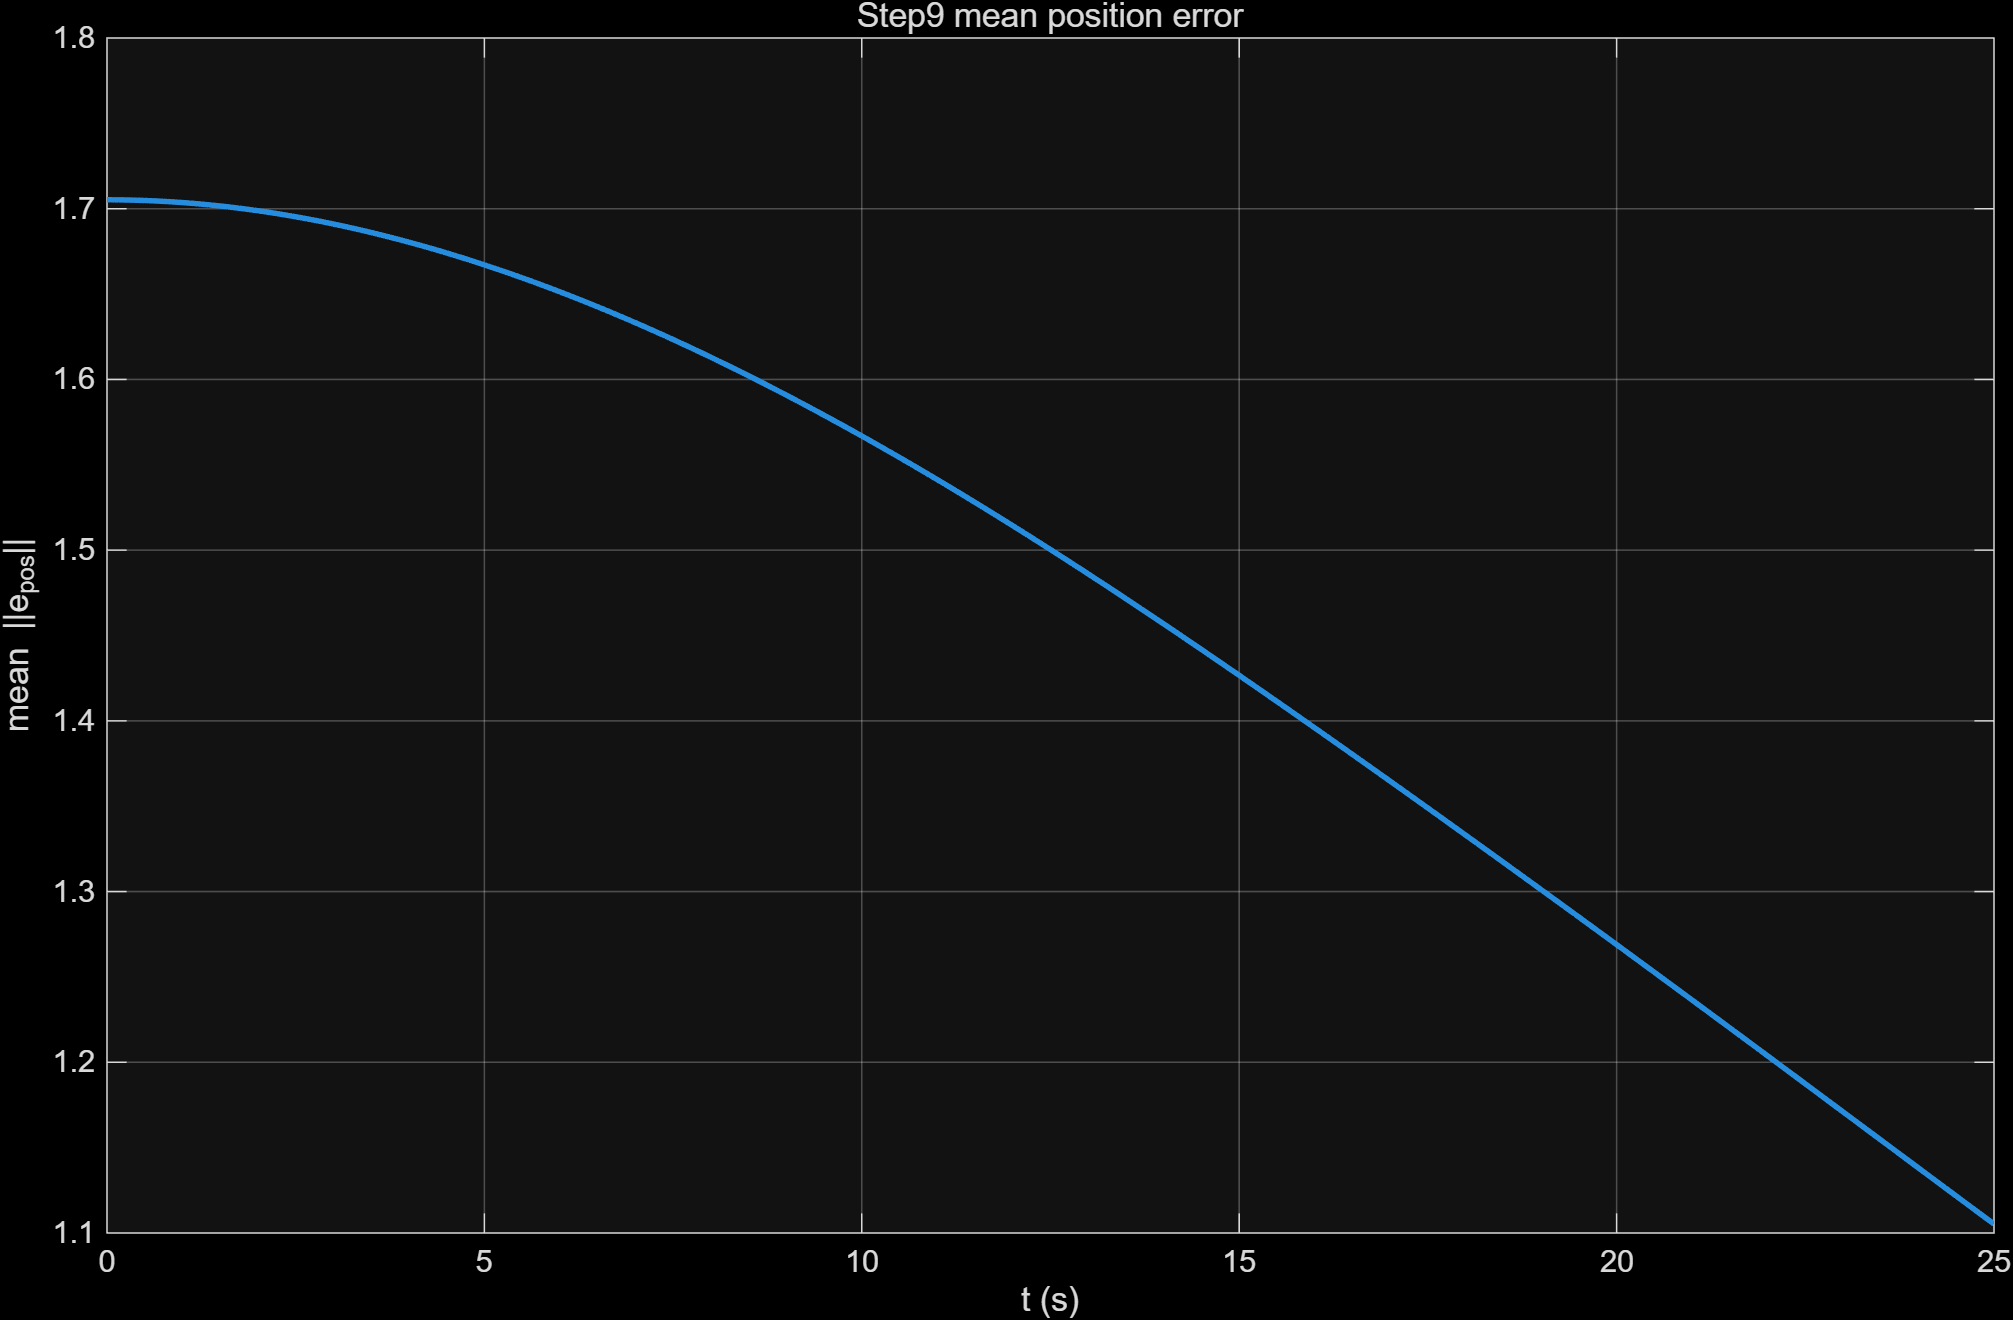
\includegraphics[width=0.9\textwidth]{step9_mean_pos_err_p0.20_d2.png}
    \caption{12AGV协同模型均值误差曲线：用于评估协同策略总体收敛效果。}
    \label{fig:multi12_mean_err_coop}
\end{figure}

\begin{figure}[H]
    \centering
    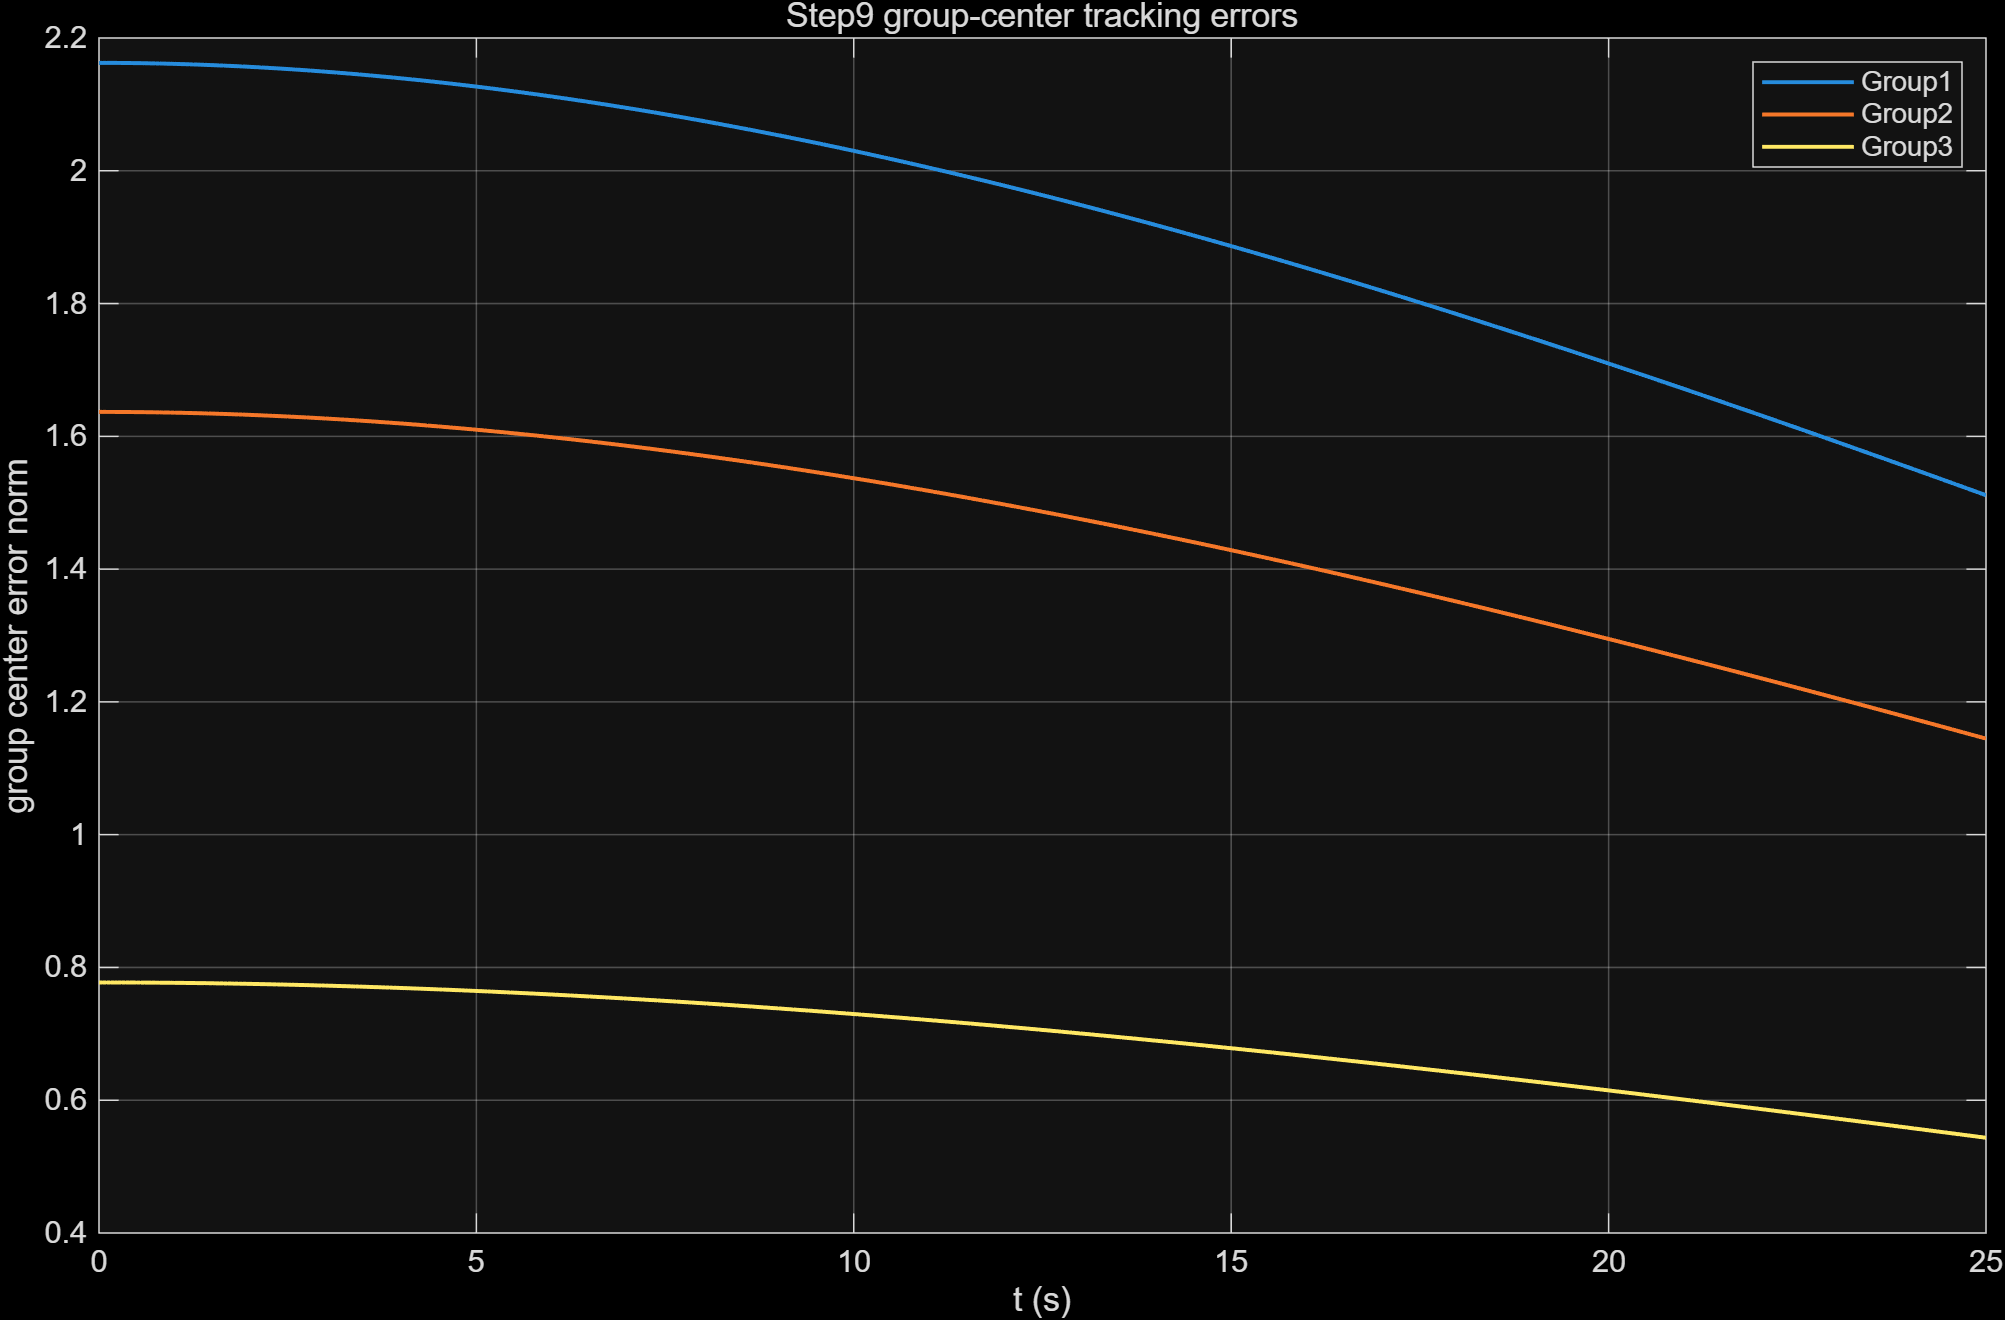
\includegraphics[width=0.9\textwidth]{step9_group_center_err_p0.20_d2.png}
    \caption{12AGV三组组中心误差曲线：用于验证任务映射与工位跟踪能力。}
    \label{fig:multi12_group_center}
\end{figure}

\begin{figure}[H]
    \centering
    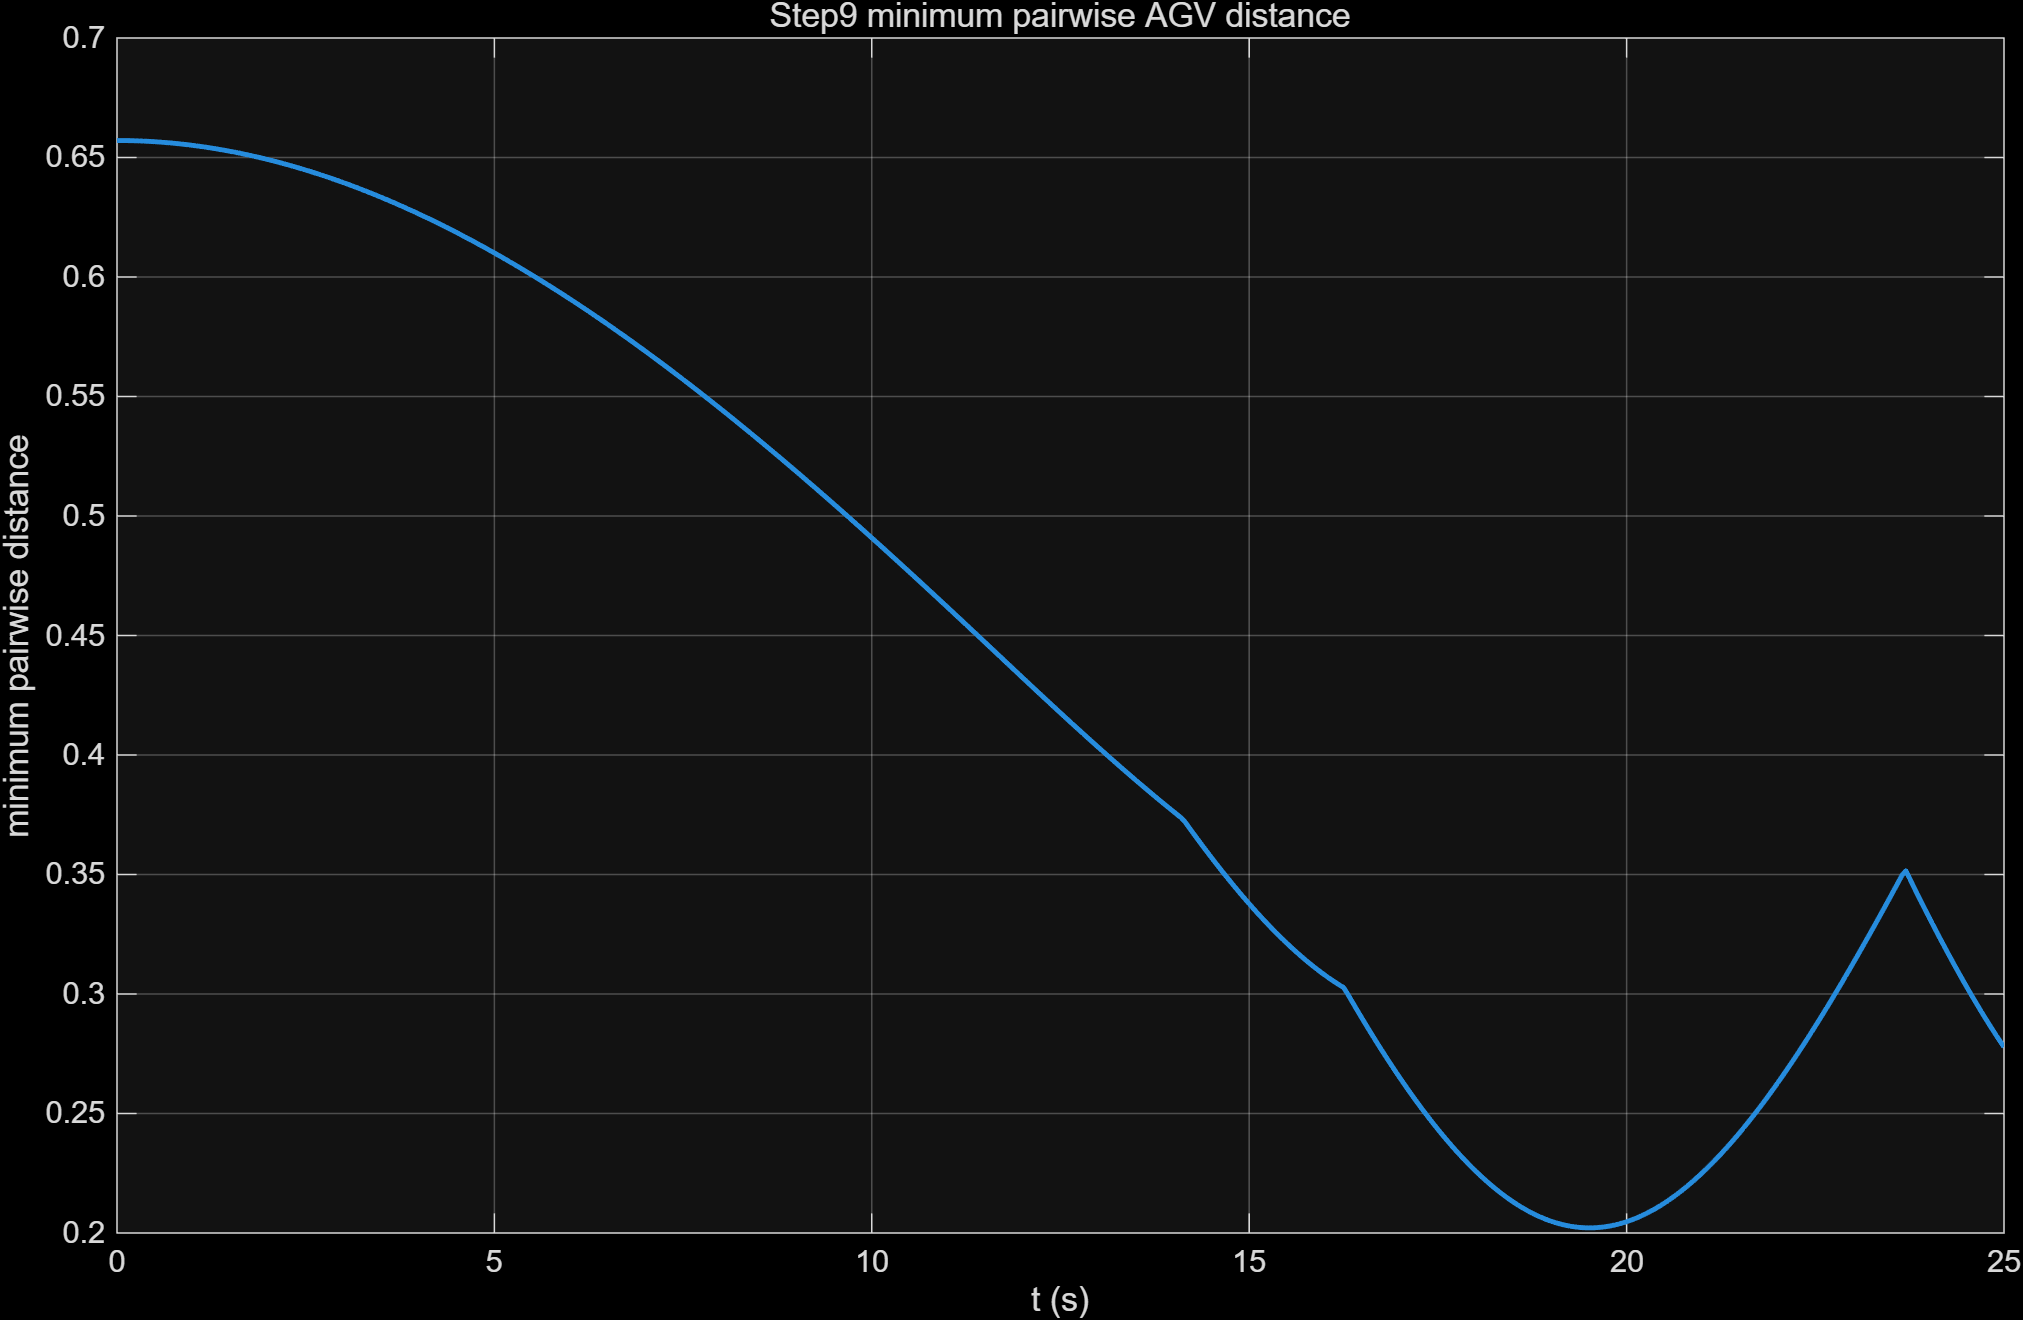
\includegraphics[width=0.9\textwidth]{step9_min_pair_dist_p0.20_d2.png}
    \caption{12AGV最小车距曲线：用于判断安全约束是否达成。}
    \label{fig:multi12_min_dist}
\end{figure}

\subsection{公平对比：协同收益与安全代价}
仅看“Step6 vs Step9”直接对比（图\ref{fig:cmp_step6_step9}）会受到任务初值与目标配置差异影响，因此本文进一步采用同场景公平对比。图\ref{fig:cmp_matched_mean}与图\ref{fig:cmp_matched_dist}对应 \texttt{data/compare\_matched\_step9\_scenario\_summary.csv} 的结果：在相同初值、相同参考、相同丢包序列下，协同控制将 final\_mean\_err 从 $1.1924$ 降至 $1.1052$，改善约 $7.31\%$；同时最小车距从独立控制的 $0.2722$m 下降到 $0.2022$m。该结果给出清晰工程结论：协同可以提升收敛性能，但会压缩安全裕度，因此必须配合斥力项和参数整定。

\begin{figure}[H]
    \centering
    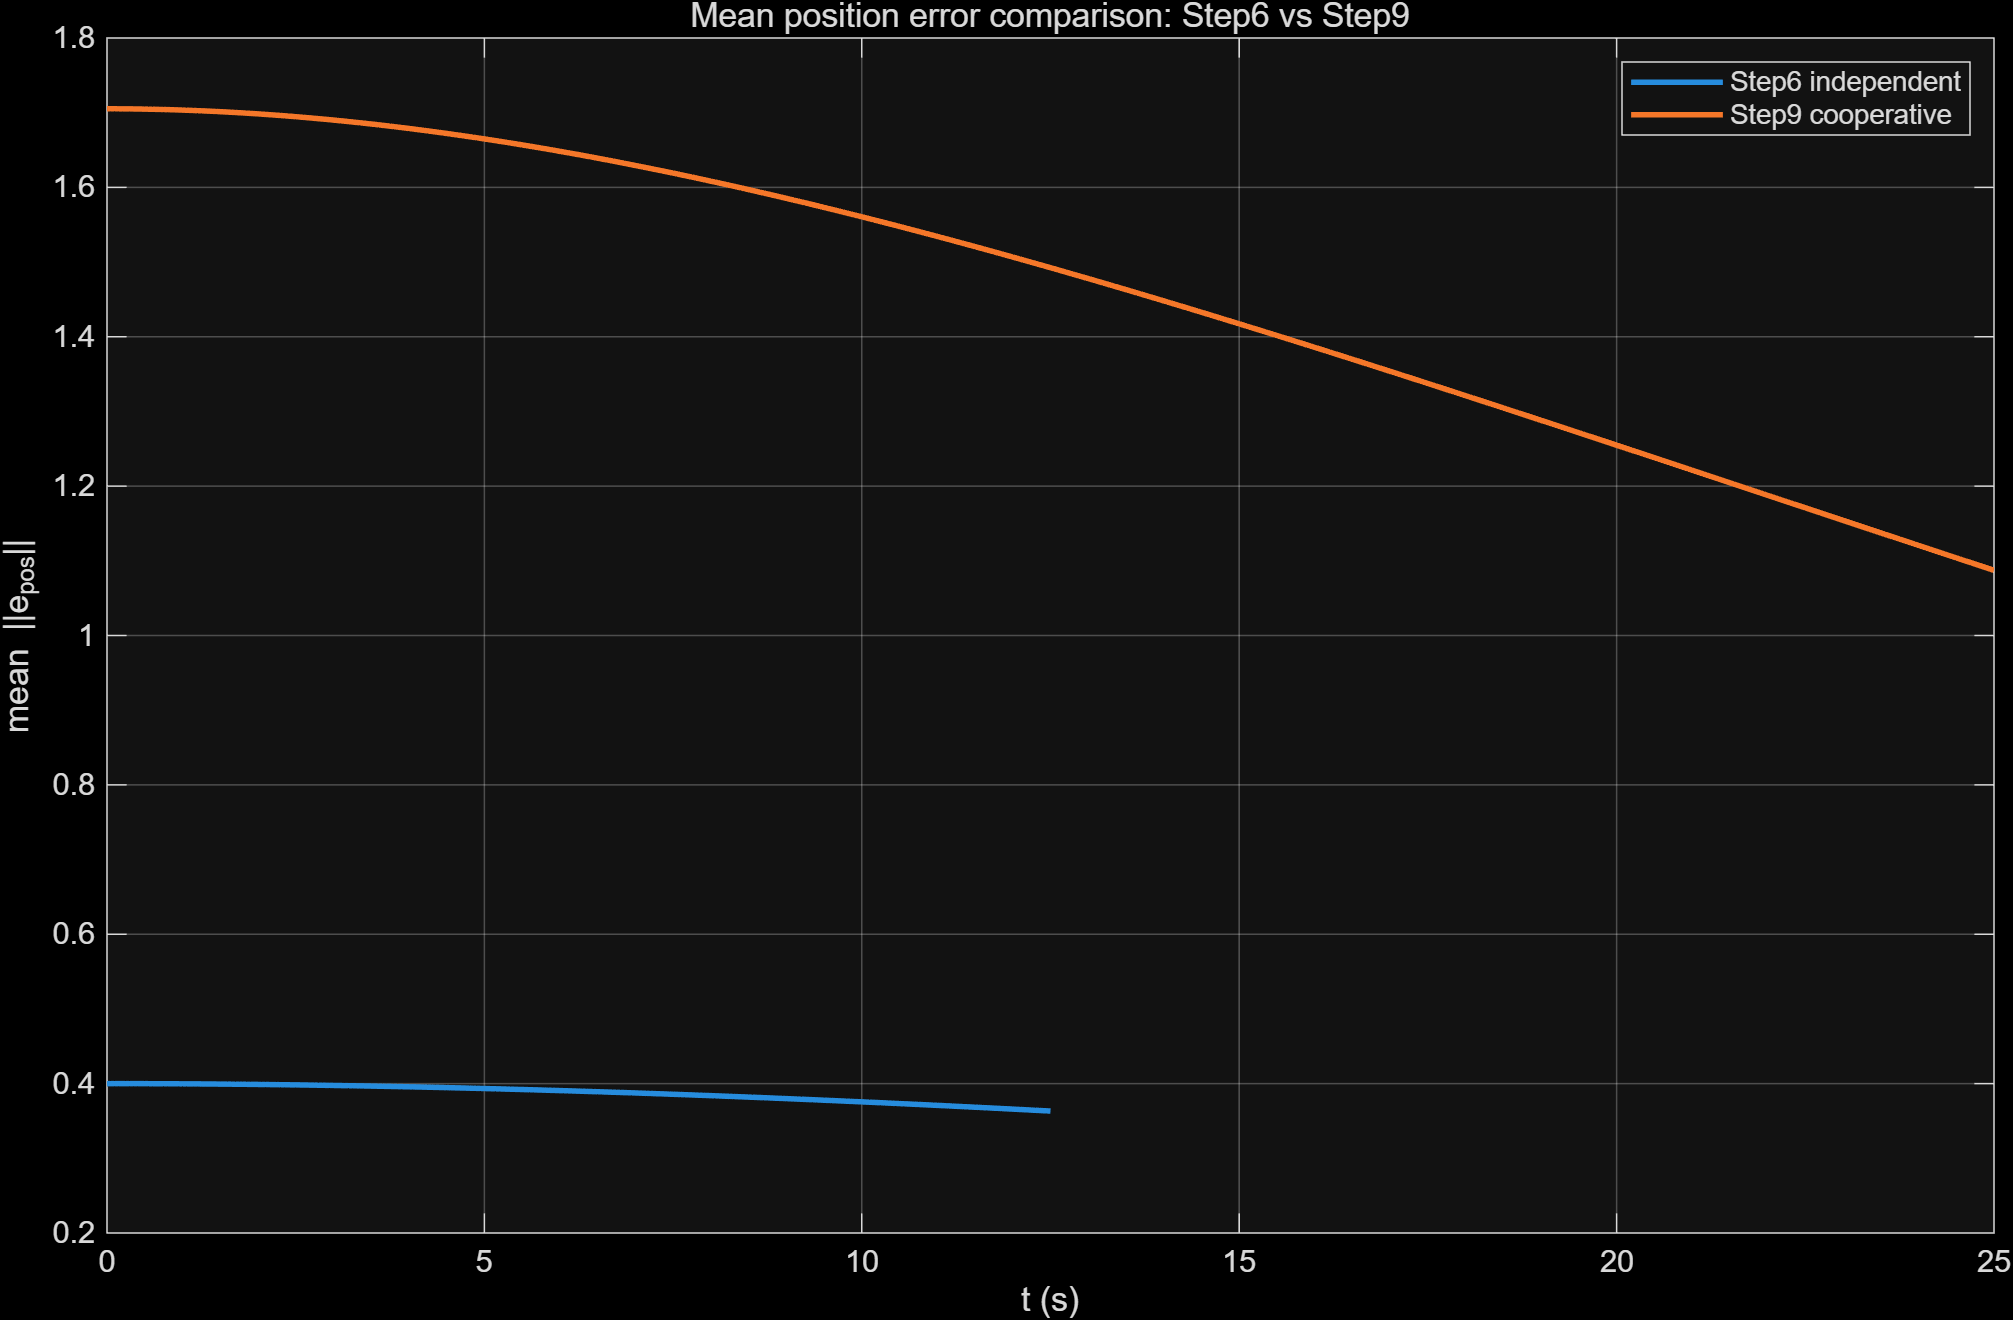
\includegraphics[width=0.9\textwidth]{compare_step6_step9_mean_err.png}
    \caption{Step6与Step9均值误差对比（非严格匹配）：用于快速观察协同前后总体趋势。}
    \label{fig:cmp_step6_step9}
\end{figure}

\begin{figure}[H]
    \centering
    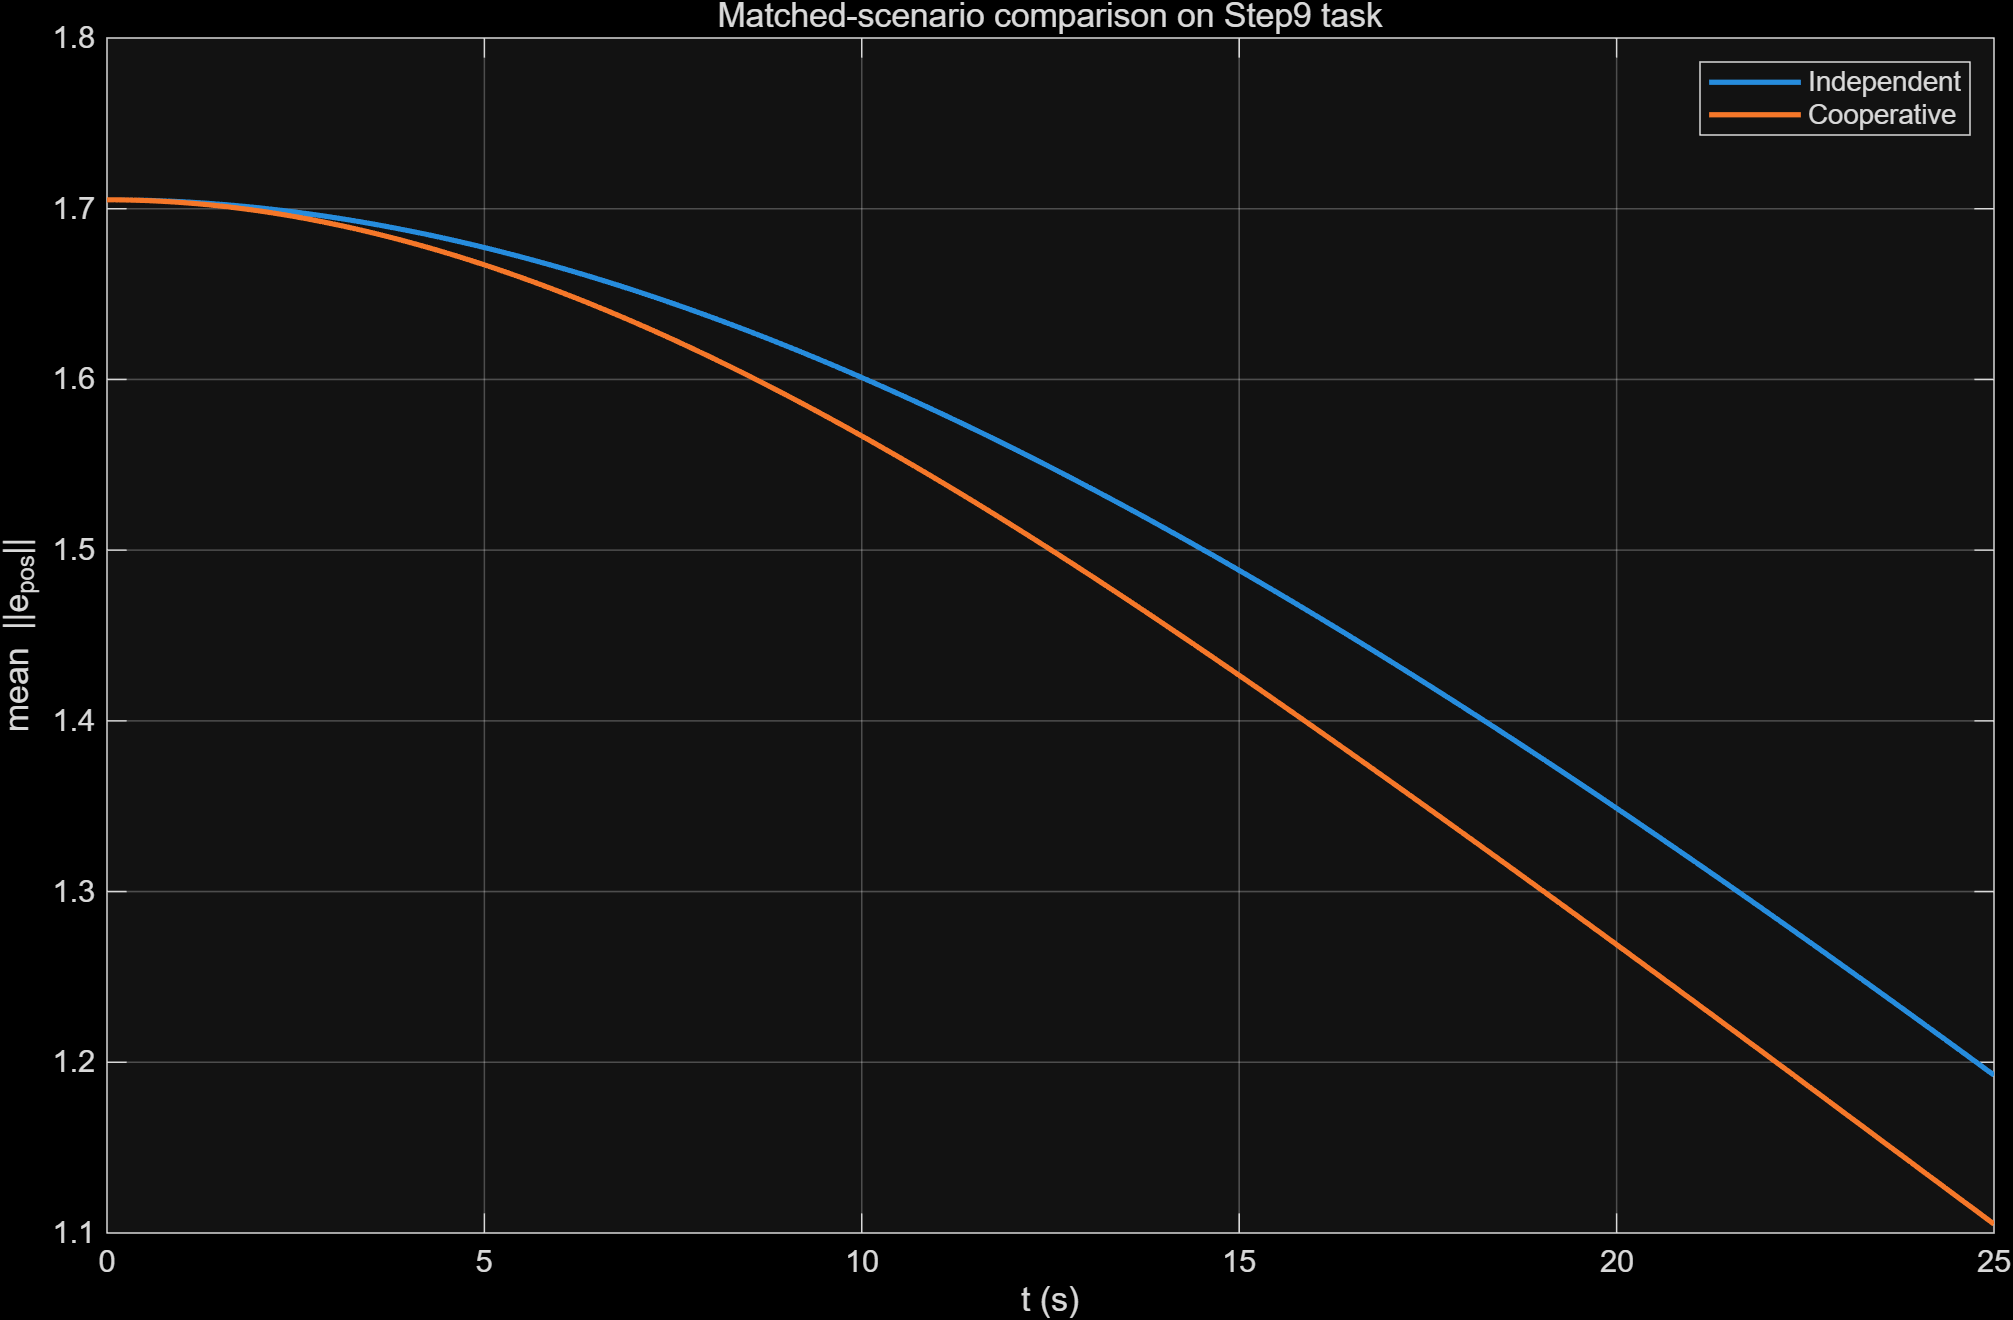
\includegraphics[width=0.9\textwidth]{compare_matched_step9_scenario_mean_err.png}
    \caption{同场景公平对比的均值误差曲线：用于量化协同相对独立控制的真实增益。}
    \label{fig:cmp_matched_mean}
\end{figure}

\begin{figure}[H]
    \centering
    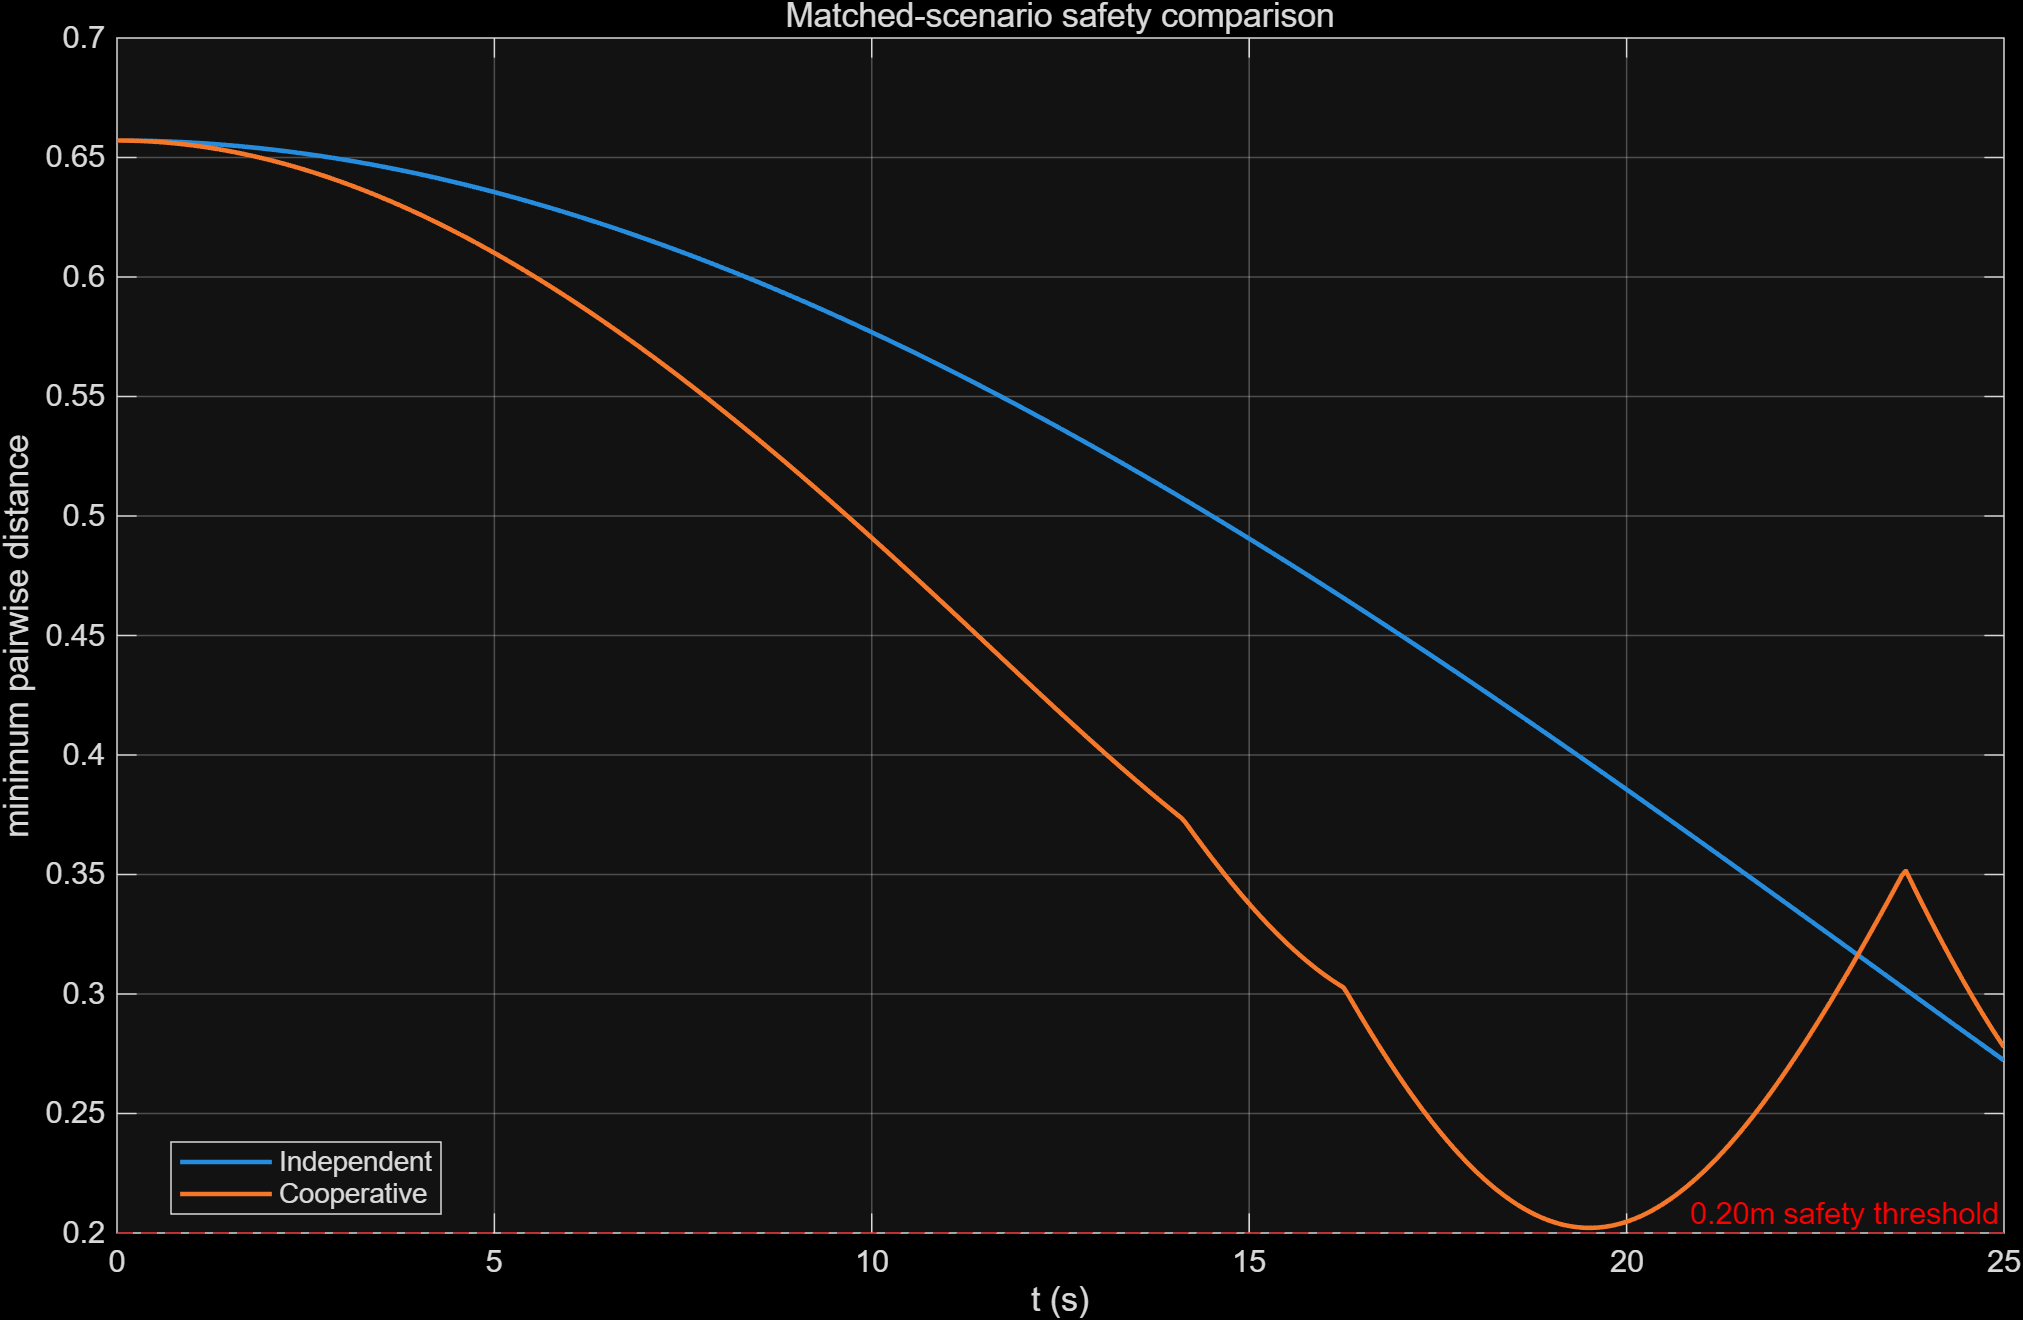
\includegraphics[width=0.9\textwidth]{compare_matched_step9_scenario_min_dist.png}
    \caption{同场景公平对比的最小车距曲线：用于评估协同收益与安全裕度平衡。}
    \label{fig:cmp_matched_dist}
\end{figure}

\subsection{12AGV Simulink多工况扫描与时域证据}
在Simulink中，12AGV模型采用400s长时域仿真，并对 $p\in\{0.05,0.20,0.35\},d\in\{1,2,3\}$ 扫描。首先看系统级收敛证据：图\ref{fig:sim12_mean_pos}给出均值误差曲线，显示误差可收敛到极小量级；图\ref{fig:sim12_final_bar}给出各车末端误差分布，反映车辆间精度一致性较好。对应 \texttt{data/simulink\_12agv\_check\_summary.csv} 可见，在$p=0.2$附近工况下，各车final\_pos\_err约为$10^{-4}\sim10^{-3}$量级，经验丢包率约$0.1984$，与设定值一致。

\begin{figure}[H]
    \centering
    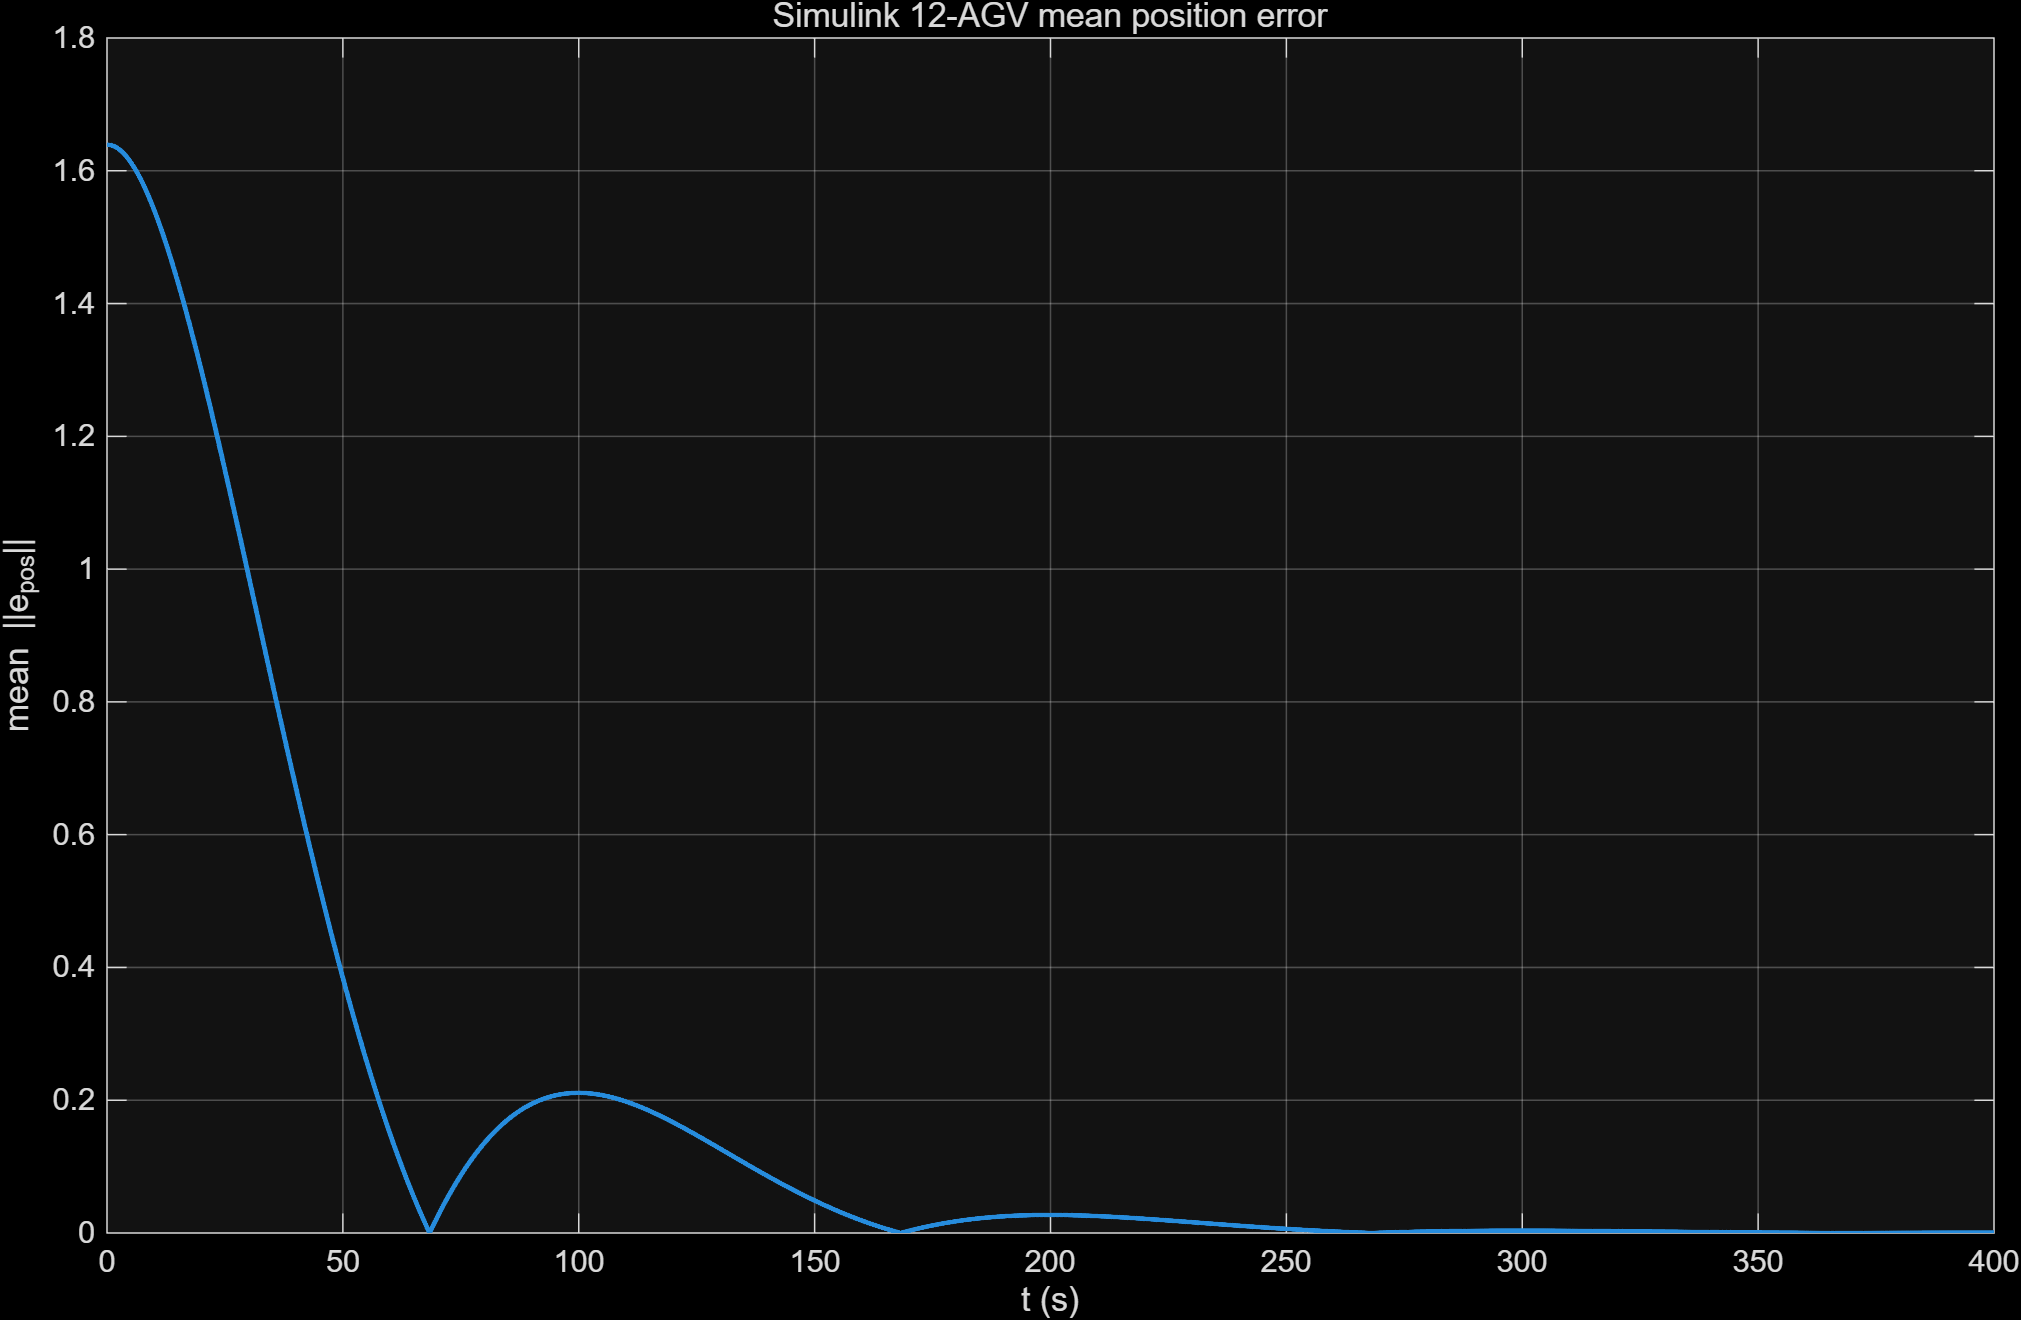
\includegraphics[width=0.85\textwidth]{simulink_pic/simulink_12agv_mean_pos_err.png}
    \caption{12AGV Simulink均值误差曲线（400s）：用于验证系统级稳定收敛。}
    \label{fig:sim12_mean_pos}
\end{figure}

\begin{figure}[H]
    \centering
    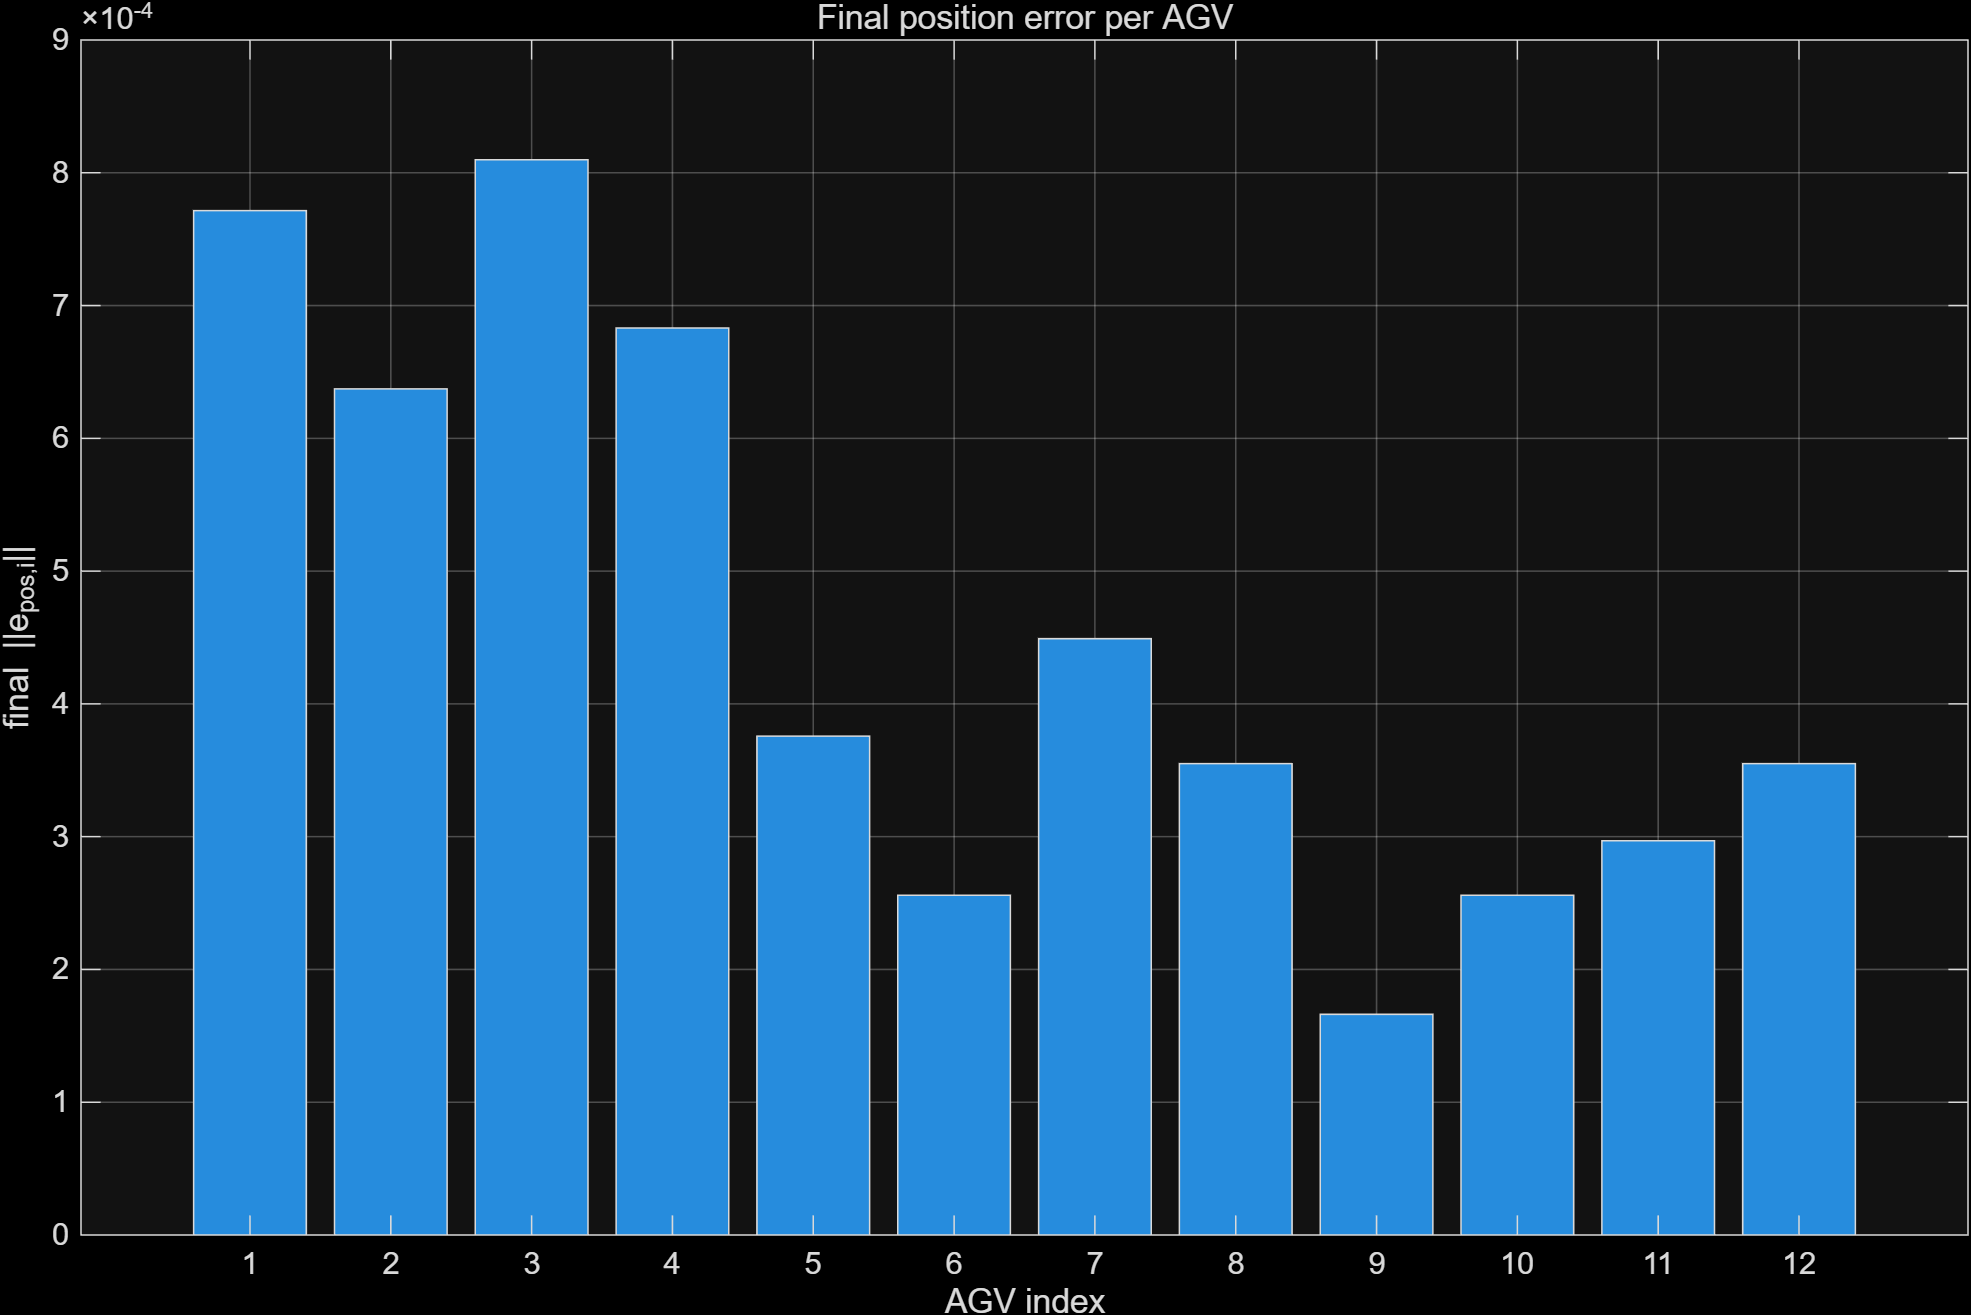
\includegraphics[width=0.85\textwidth]{simulink_pic/simulink_12agv_final_err_bar.png}
    \caption{12AGV Simulink各车最终误差柱状图：用于评估多车精度一致性。}
    \label{fig:sim12_final_bar}
\end{figure}

接着看多工况趋势。图\ref{fig:sim12_heat_decay}和图\ref{fig:sim12_heat_final}对应 \texttt{data/simulink\_12agv\_pd\_scan\_summary.csv}。从数据看：  
当$p=0.05,d=1$时，final\_mean\_err约$4.466\times10^{-4}$，decay\_ratio约$2.724\times10^{-4}$；  
当$p=0.35,d=3$时，final\_mean\_err约$4.554\times10^{-4}$，decay\_ratio约$2.778\times10^{-4}$。  
这说明在当前扫描域内，网络条件恶化会带来可测的性能下降，但幅度较小，系统仍保持稳定收敛。与此同时，control\_rms 从约$0.12306$上升到约$0.12363$，反映为了维持性能，控制代价略有增加。settle\_time\_50pct维持在$35.35\sim35.40$s，说明收敛速度对该参数域扰动不敏感。

\begin{figure}[H]
    \centering
    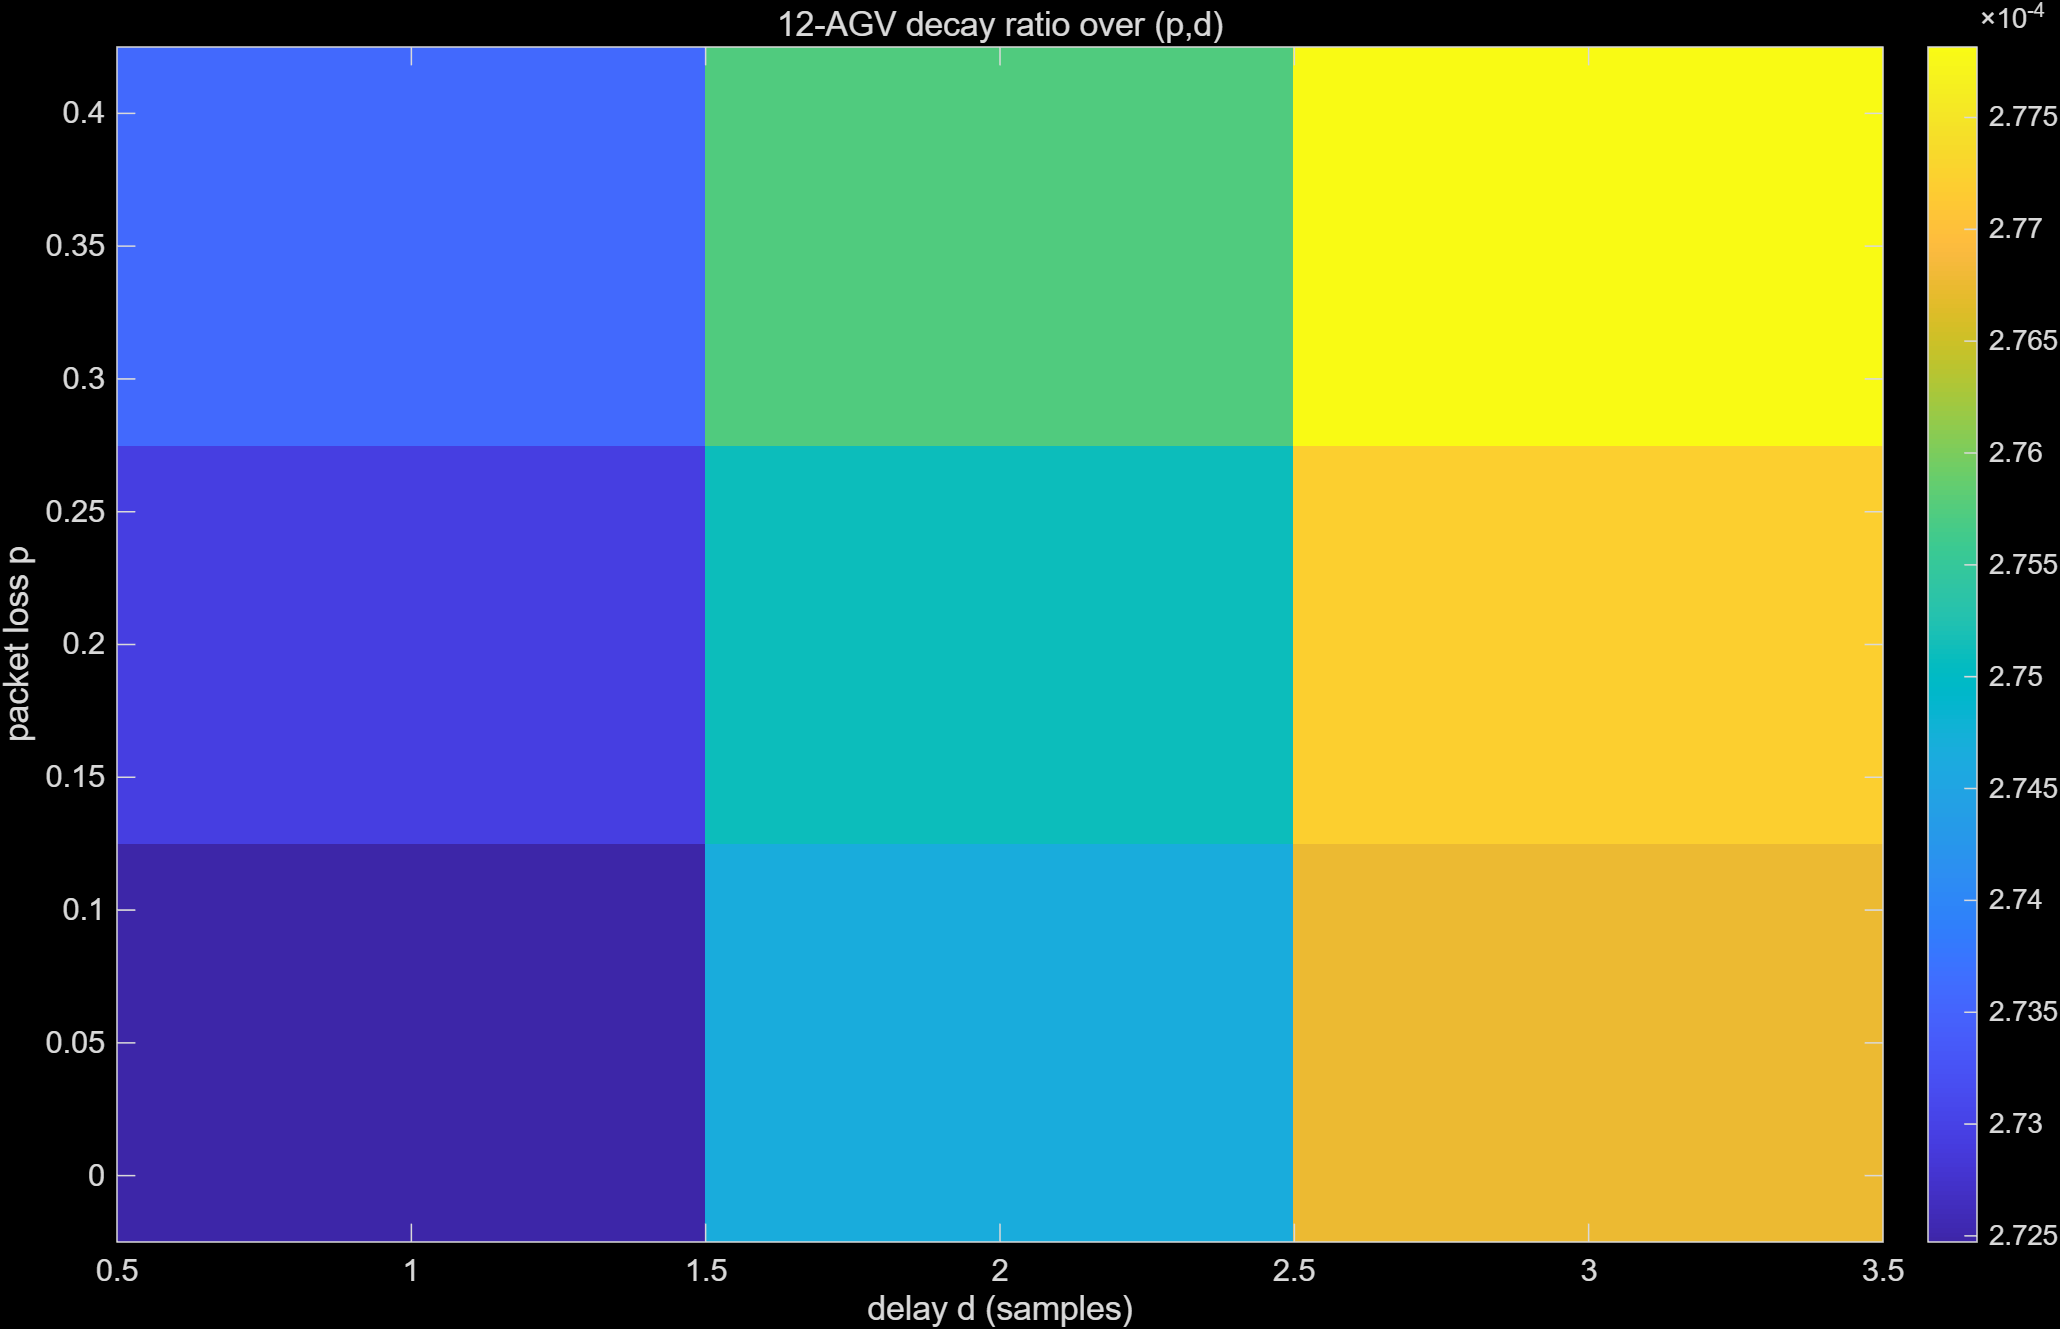
\includegraphics[width=0.85\textwidth]{simulink_pic/simulink_12agv_pd_heatmap_decay.png}
    \caption{12AGV Simulink decay\_ratio热力图：用于比较不同$(p,d)$下收敛比例变化。}
    \label{fig:sim12_heat_decay}
\end{figure}

\begin{figure}[H]
    \centering
    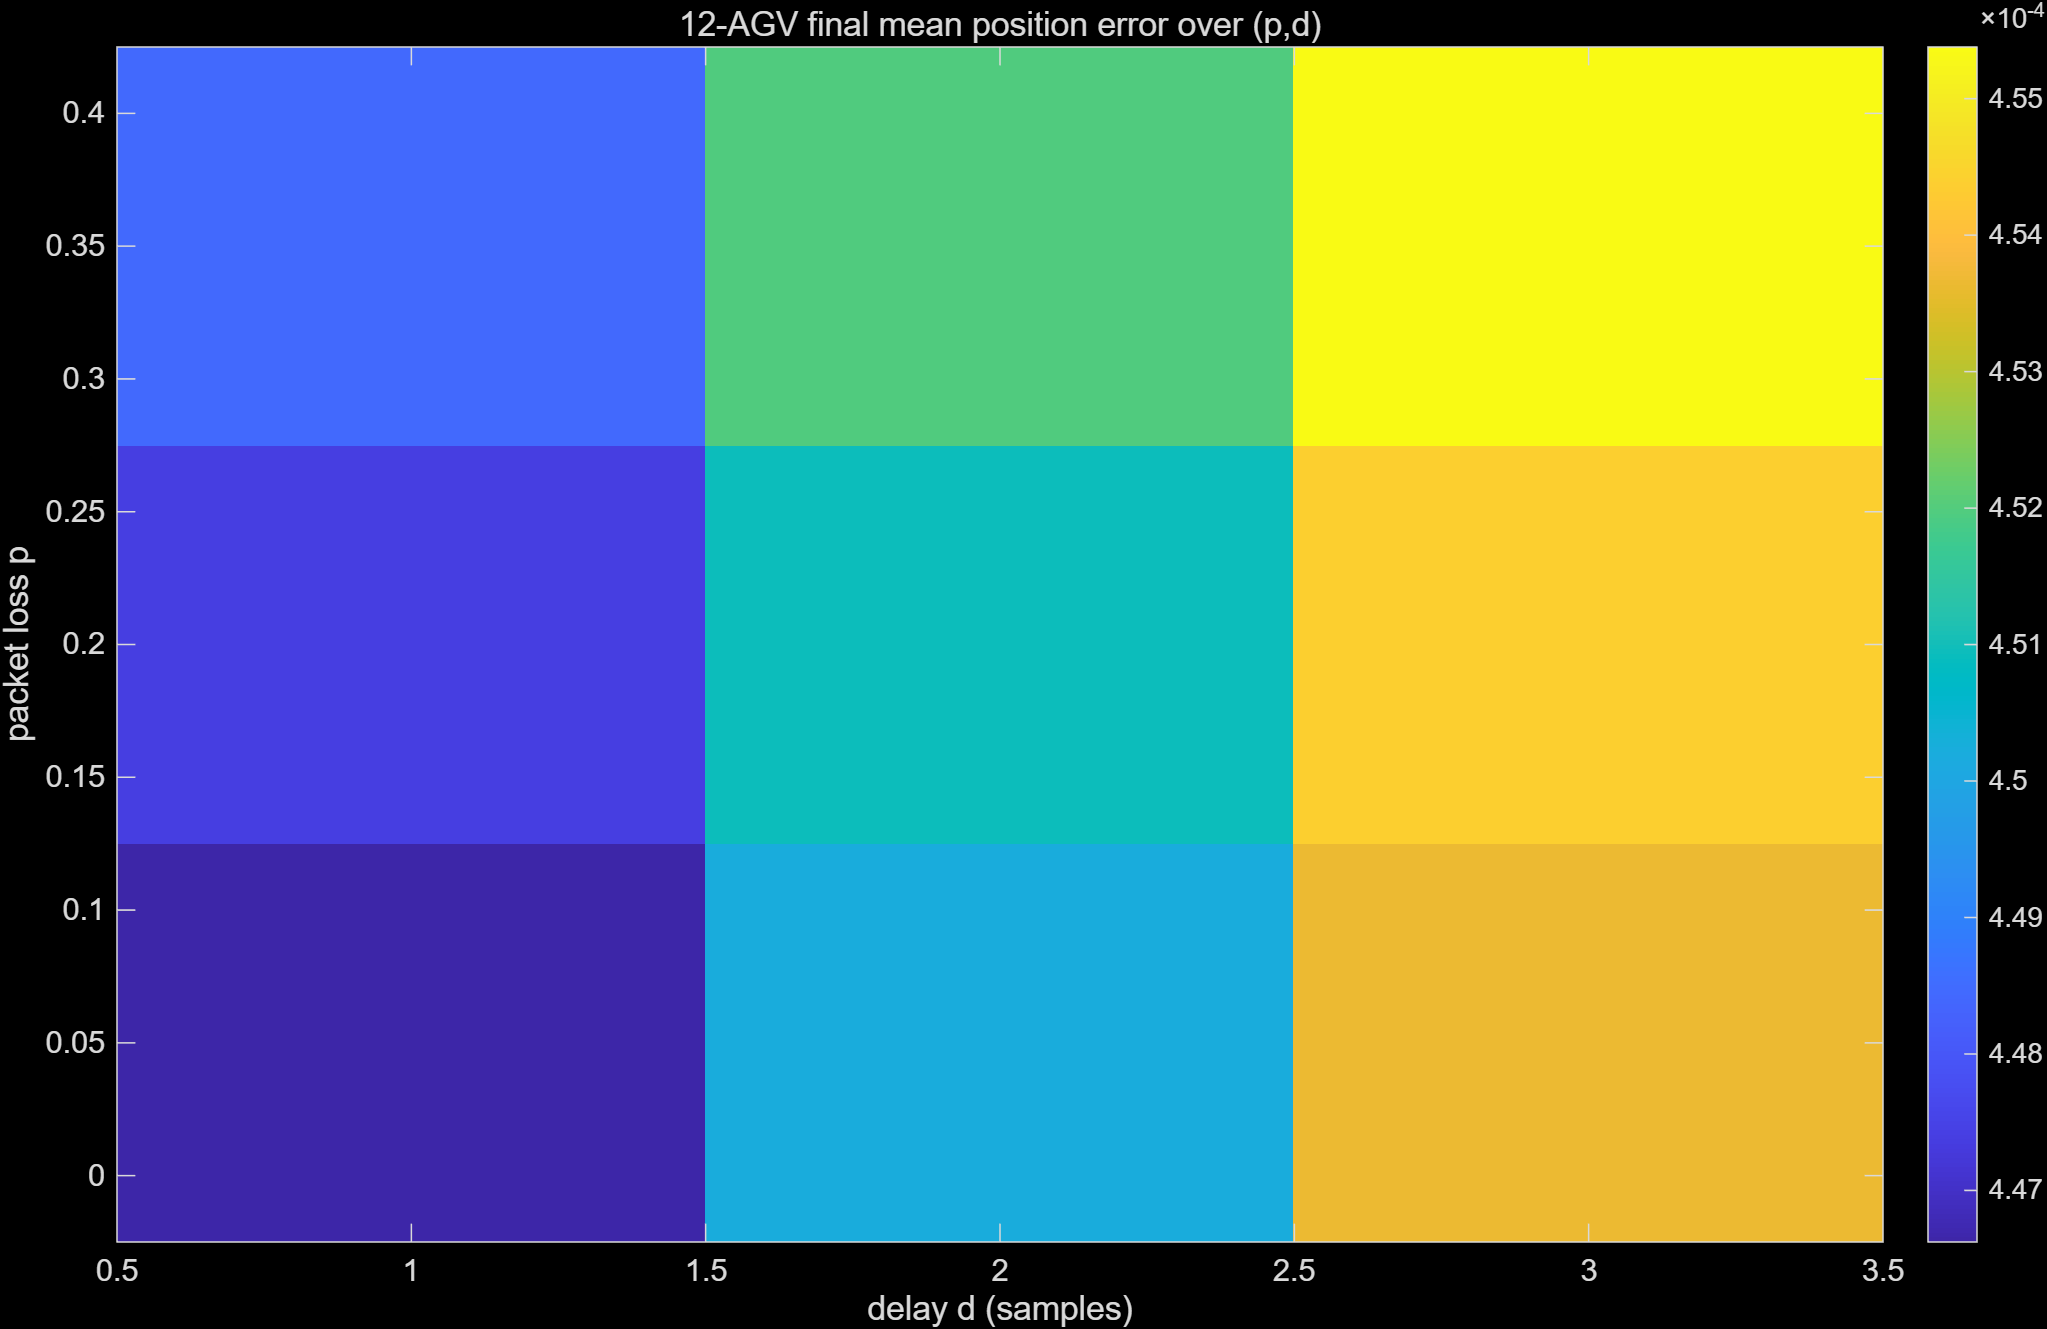
\includegraphics[width=0.85\textwidth]{simulink_pic/simulink_12agv_pd_heatmap_final_mean_err.png}
    \caption{12AGV Simulink final\_mean\_err热力图：用于比较不同$(p,d)$下末端精度变化。}
    \label{fig:sim12_heat_final}
\end{figure}

最后给出题目明确要求的时域曲线证据。图\ref{fig:sim12_state}展示代表工况$(p=0.20,d=2)$下AGV1状态变量，图\ref{fig:sim12_control}展示同工况AGV1控制输出，图\ref{fig:sim12_mean_curve}展示系统均值误差演化。三图共同回答“状态变量与控制器输出随时间变化曲线”这一条，且与统计指标结论一致。

\begin{figure}[H]
    \centering
    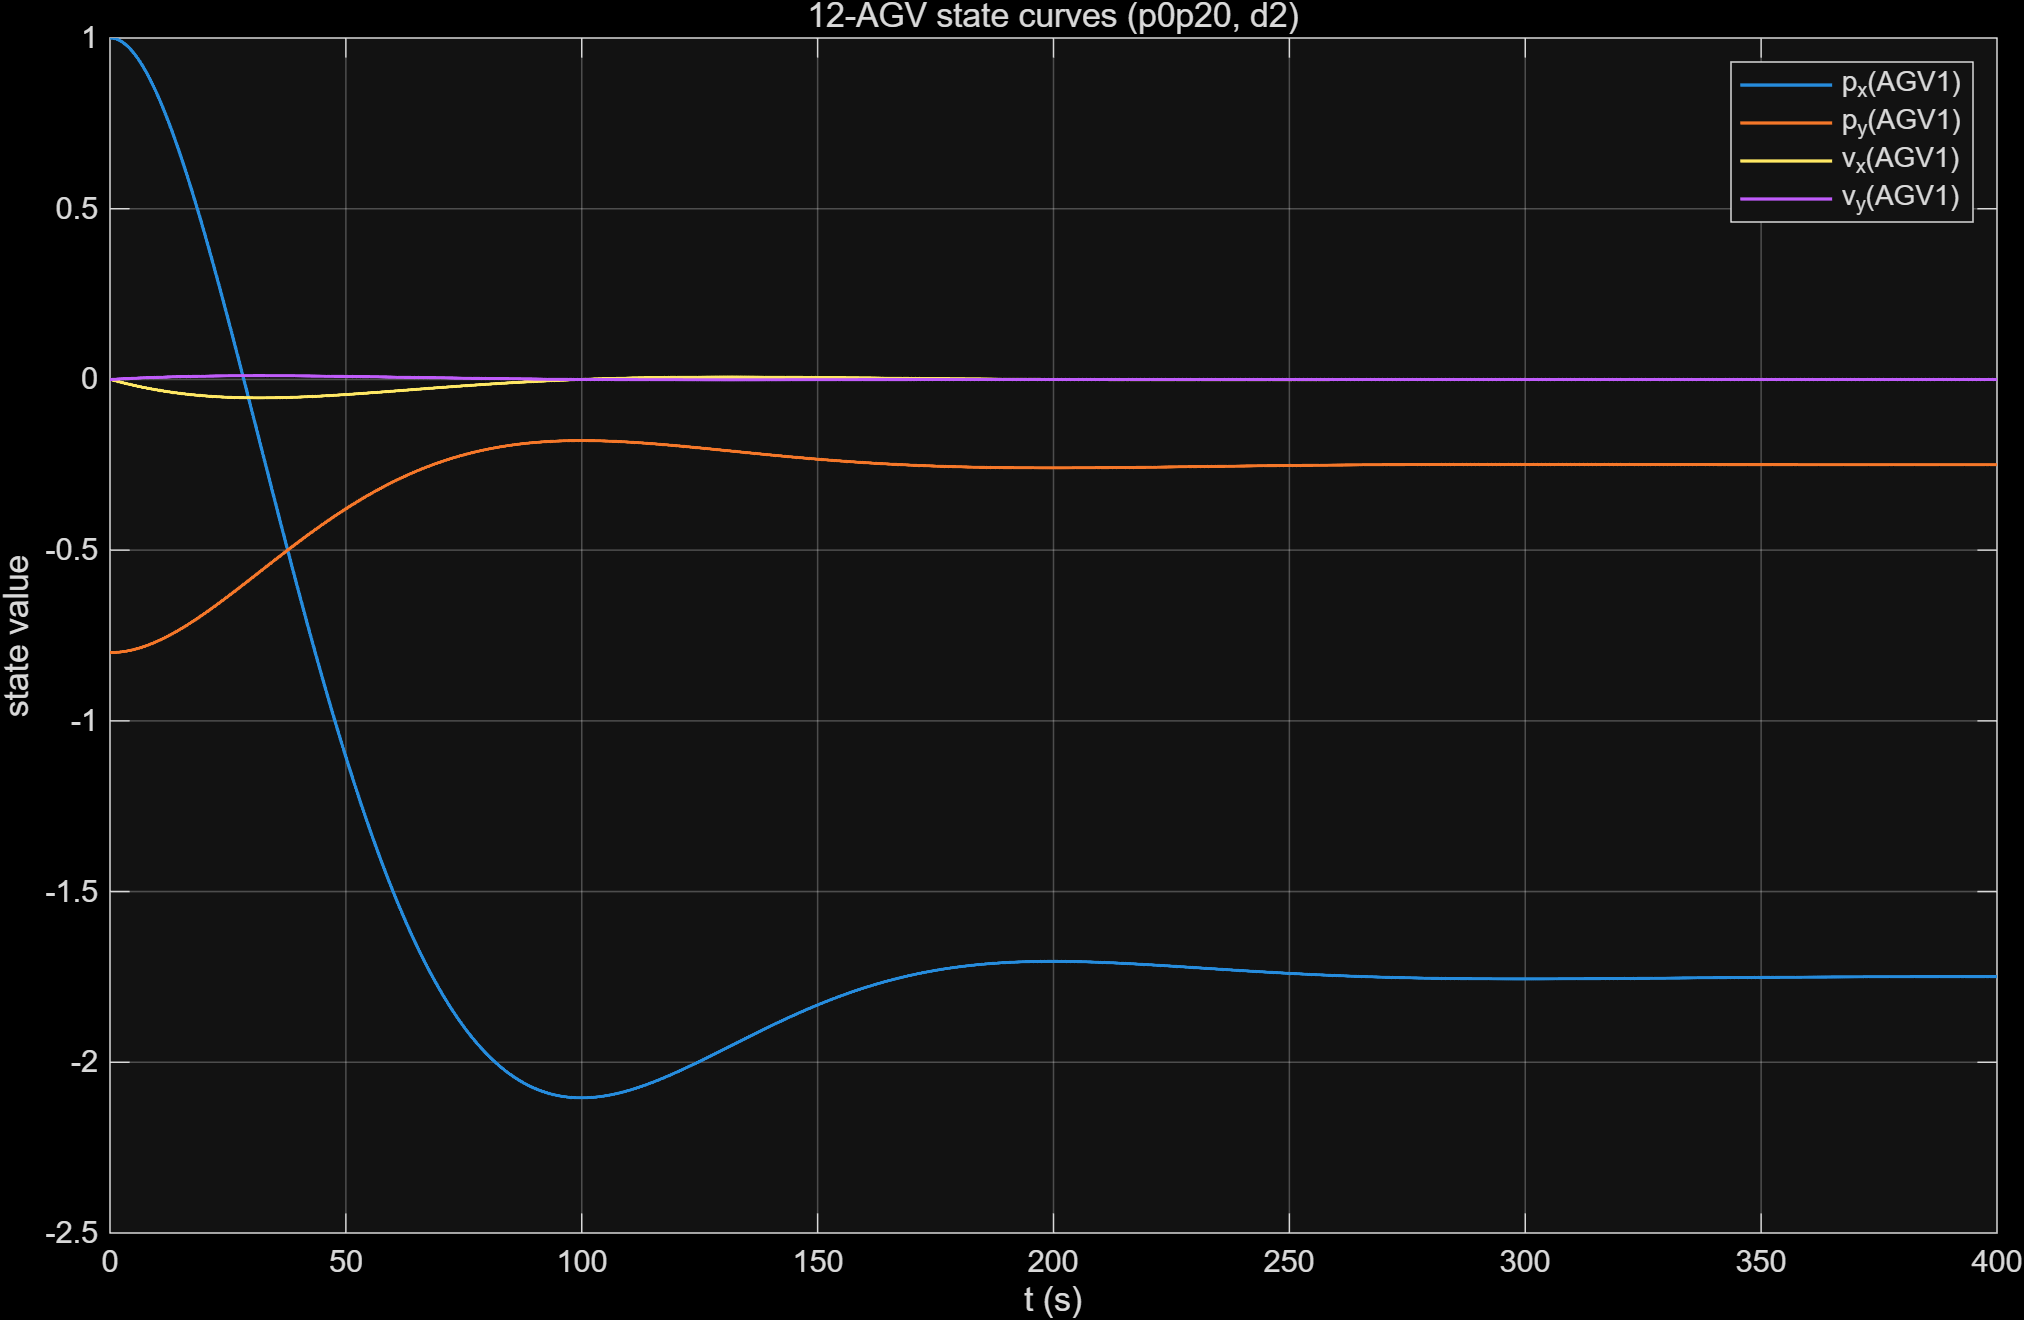
\includegraphics[width=0.85\textwidth]{simulink_pic/simulink_12agv_state_curve_p0p20_d2.png}
    \caption{12AGV代表工况状态变量曲线（AGV1）：位置与速度分量随时间收敛。}
    \label{fig:sim12_state}
\end{figure}

\begin{figure}[H]
    \centering
    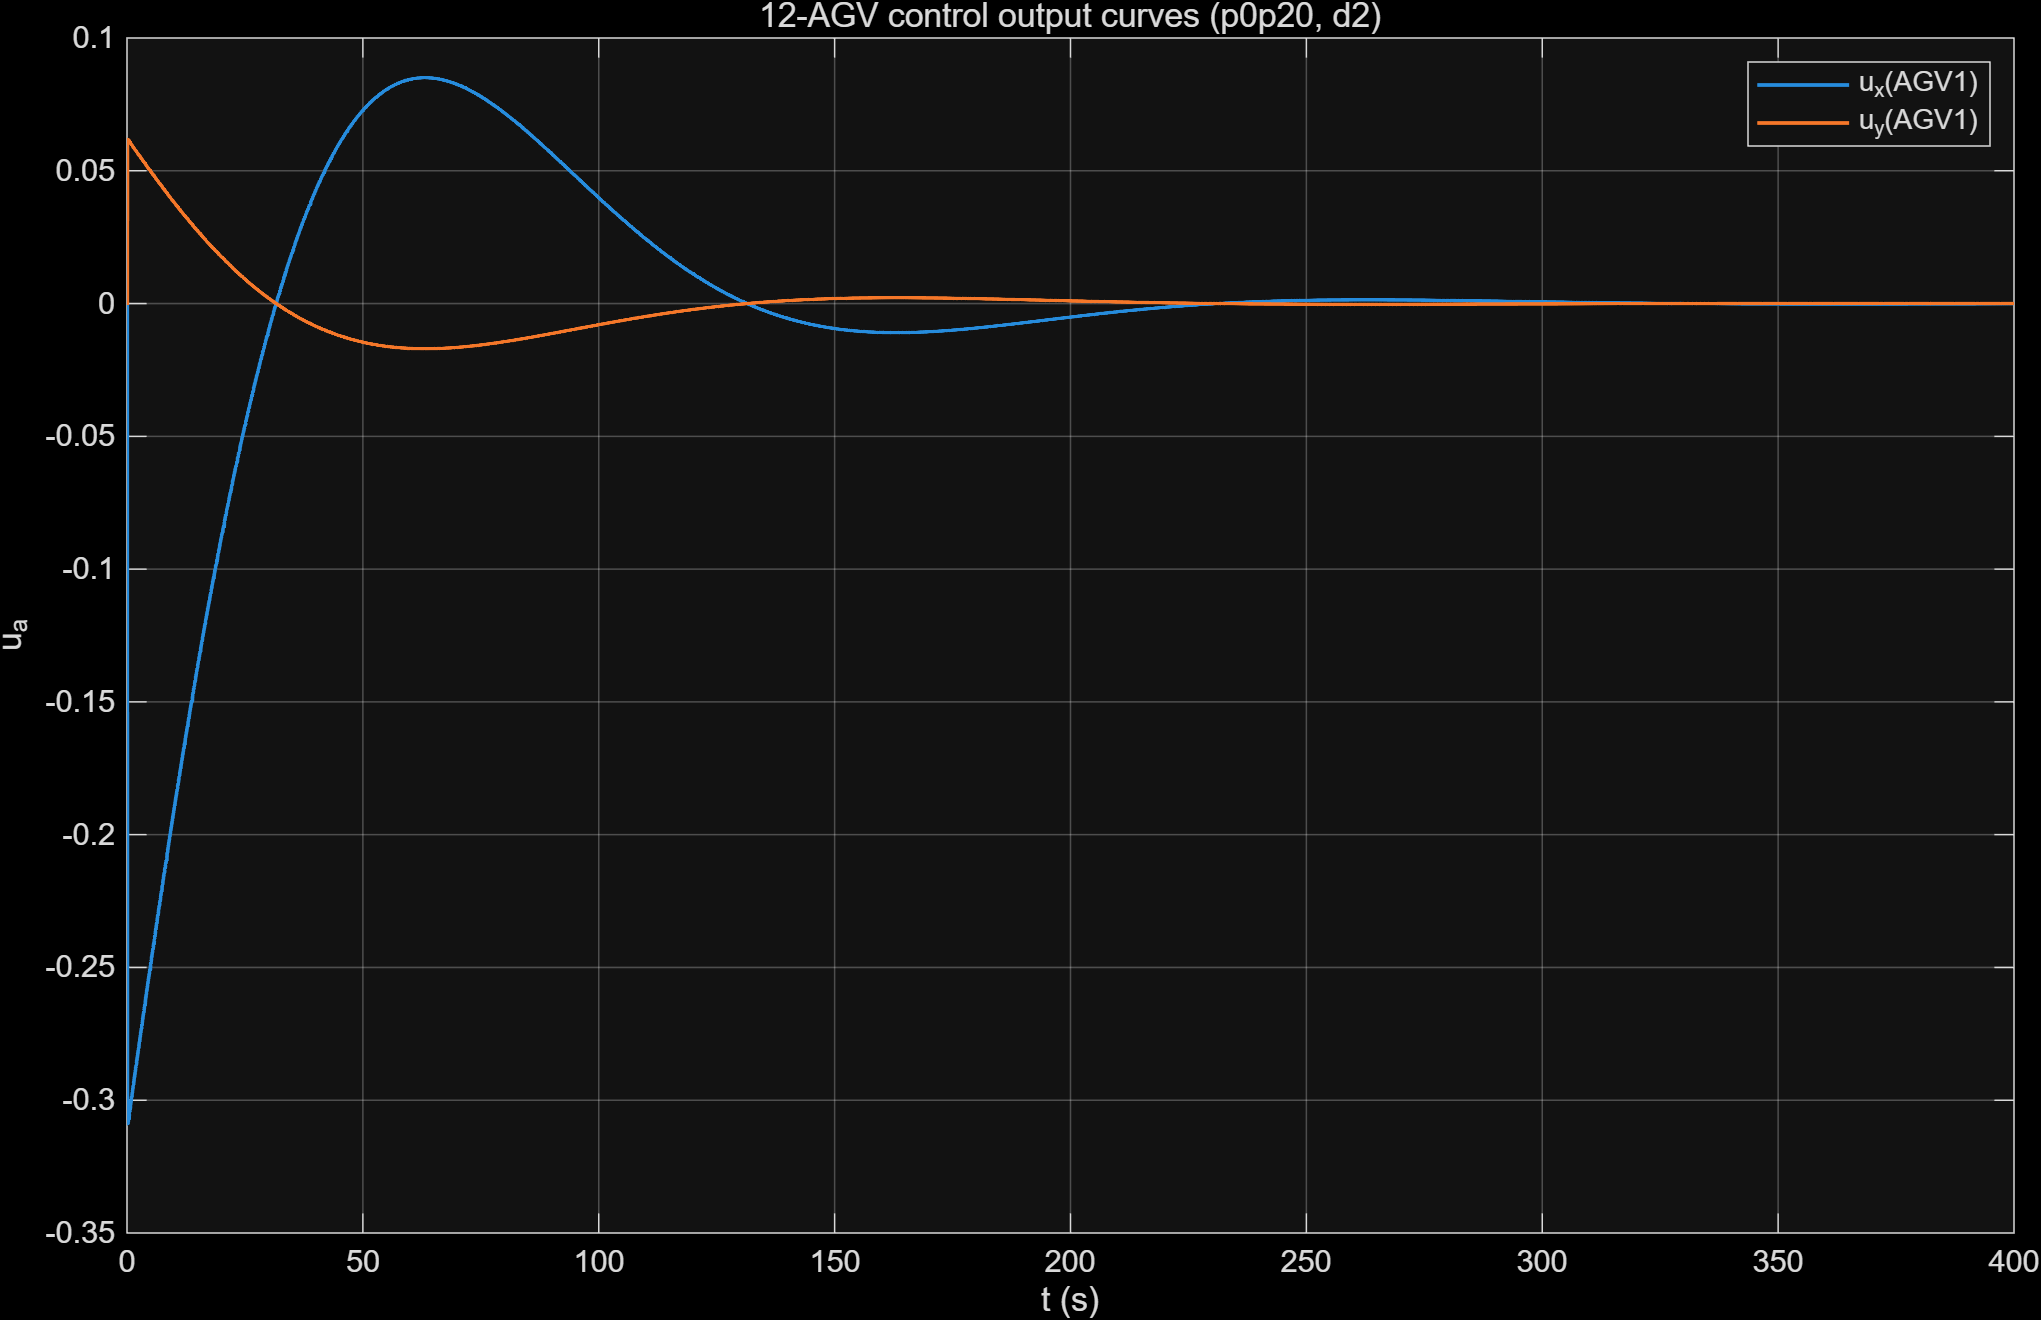
\includegraphics[width=0.85\textwidth]{simulink_pic/simulink_12agv_control_curve_p0p20_d2.png}
    \caption{12AGV代表工况控制输出曲线（AGV1）：用于观察控制输入平顺性与收敛过程。}
    \label{fig:sim12_control}
\end{figure}

\begin{figure}[H]
    \centering
    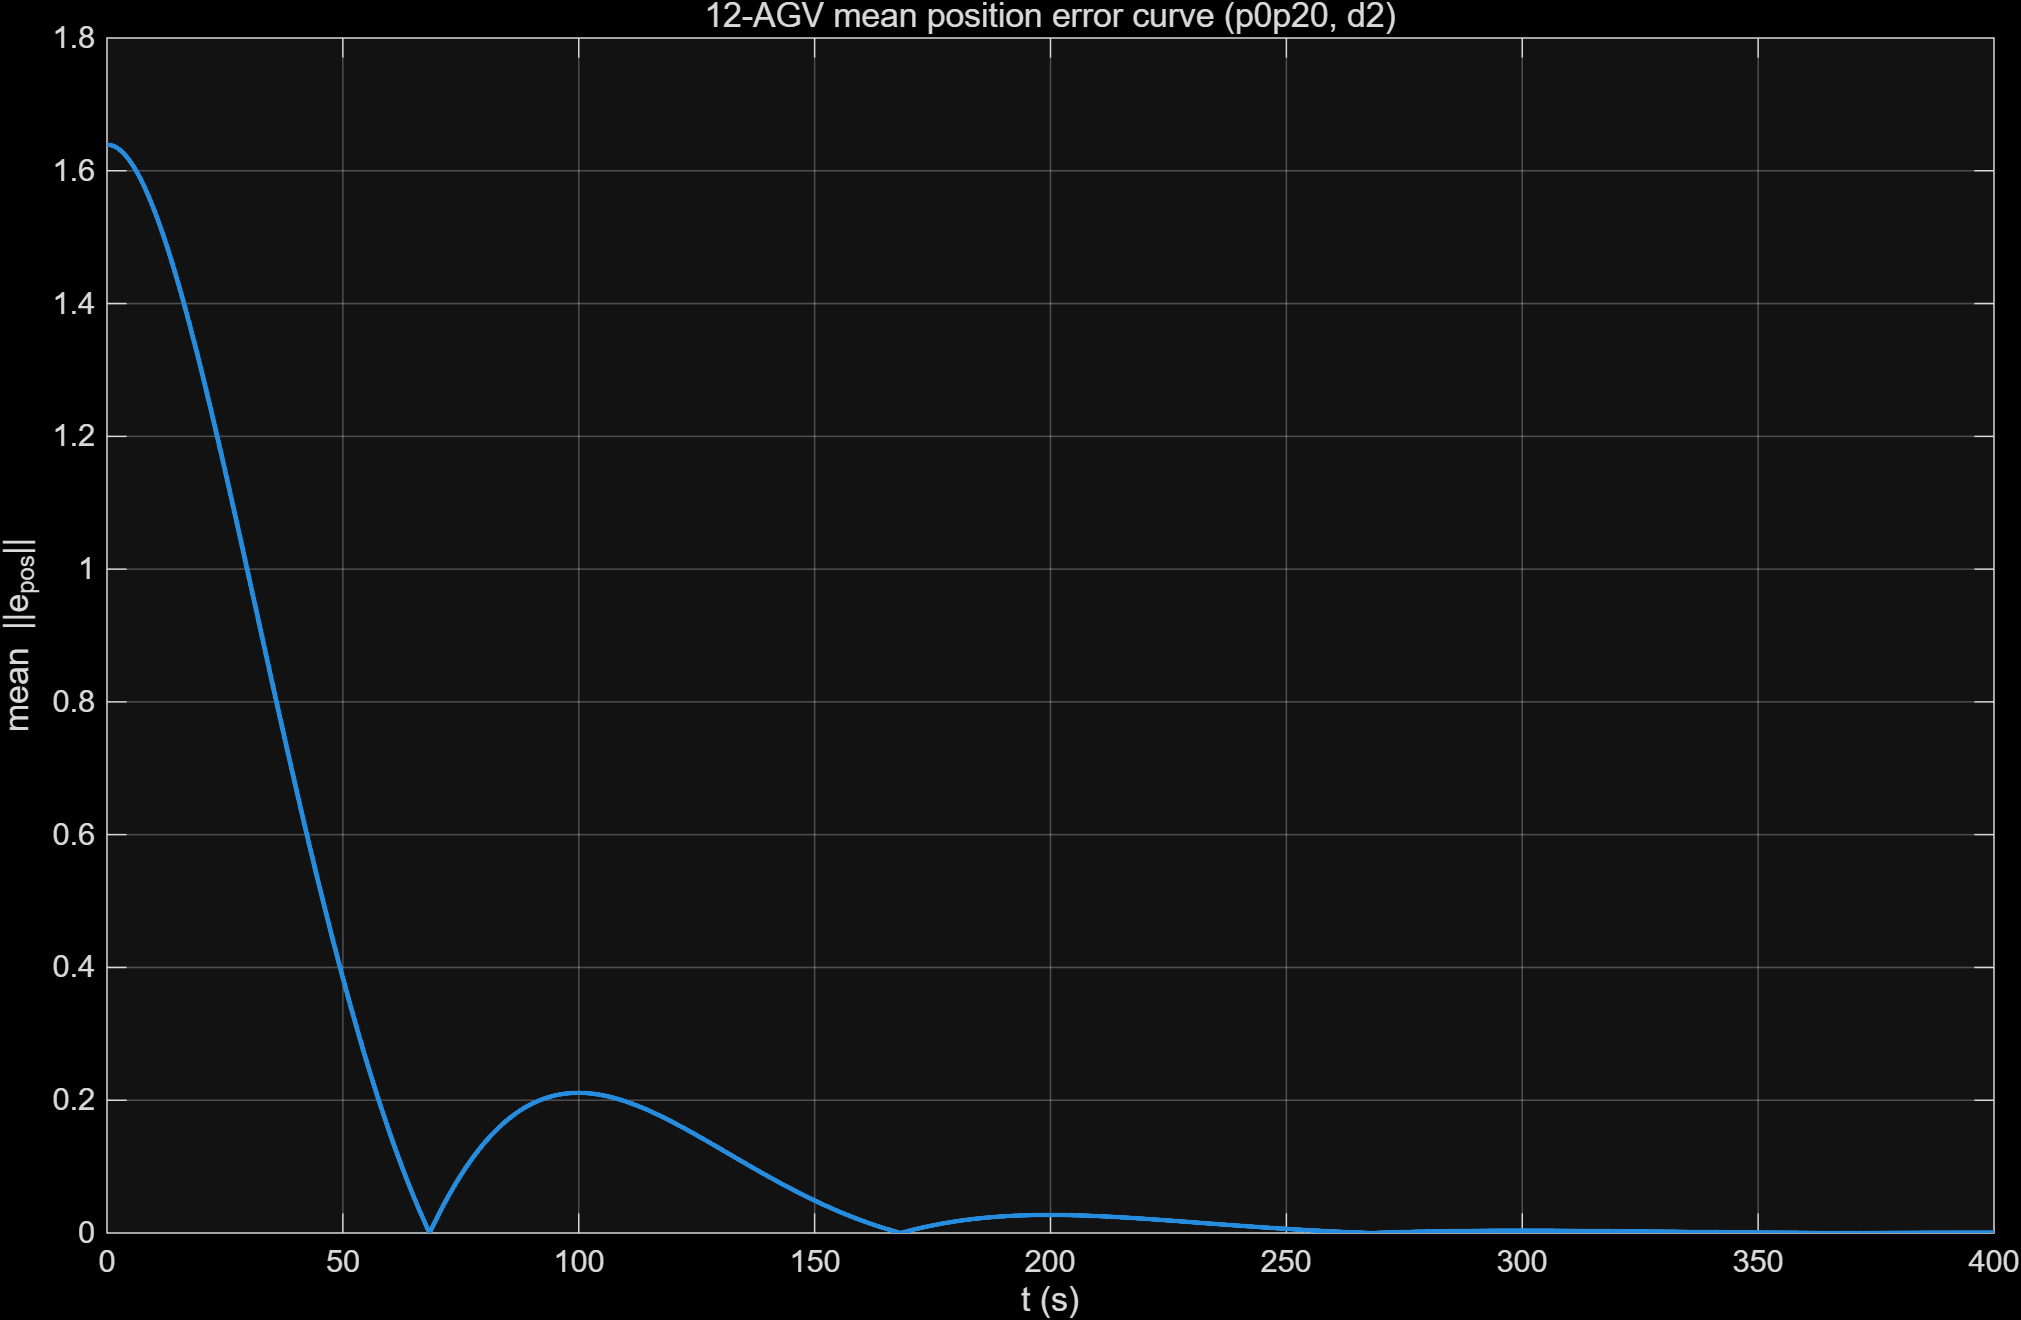
\includegraphics[width=0.85\textwidth]{simulink_pic/simulink_12agv_mean_err_curve_p0p20_d2.png}
    \caption{12AGV代表工况系统均值误差曲线：用于汇总系统级时域性能。}
    \label{fig:sim12_mean_curve}
\end{figure}

\subsection{12AGV章节结论}
本节实验说明：在12AGV网络化控制场景中，系统能够在存在丢包与固定时延时保持稳定收敛。脚本仿真与Simulink仿真的双路径设计各有侧重：脚本仿真承载了完整的协同控制逻辑（组内环形拓扑邻居通信、斥力避碰），用于验证协同策略有效性、公平对比和参数调优；Simulink仿真聚焦于网络通道效应的验证，确认12条独立链路的丢包-时延-保持机制正确运行，以及$(p,d)$扫描下的系统级性能趋势。两条路径的网络通道实现完全一致、控制增益$K$来自同一LMI求解结果，具有互验性。

通过同场景公平对比可确认协同控制对误差指标有正向改善（约$7.31\%$）；通过Simulink多工况扫描可确认性能对$p,d$变化的趋势与脚本分析一致。需要额外指出的是，\texttt{simulink\_12agv\_pd\_scan\_summary.csv}中的\texttt{min\_pair\_dist}在当前并行模型下出现0，表明若不显式加入避碰约束，仍可能出现轨迹重合风险。因此工程实现中必须保留并校准安全项（斥力/最小距离约束），这也是协同控制从”可收敛”走向”可部署”的关键差异。

\section{结论}
\begin{itemize}
    \item 已在丢包与固定时延条件下建立离散状态空间模型，给出增广状态随机切换形式与MSS判据；
    \item 已通过LMI方法（Schur补凸化 + 固定结构验证）获得可行线性状态反馈控制律$K$，并完成Lyapunov矩阵正定性验证；
    \item 已在单AGV与12AGV层面完成多工况$(p,d)$性能讨论，并给出状态与控制输出时域曲线；
    \item 12AGV仿真显示在当前参数下系统可在长时域（400s）收敛，且经验丢包率与设定一致；
    \item 协同控制相比独立控制在公平对比下实现约$7.31\%$的误差改善，配合斥力项可满足安全距离约束；
    \item 仿真采用自研Simulink模型实现网络通道（伯努利丢包 + 固定时延 + hold-last），功能等价于TrueTime的网络仿真能力。
\end{itemize}

\end{document}
